%!TEX program = lualatex
%!TEX encoding = UTF-8 Unicode  
%!TEX root = chapter04.tex  
\documentclass[main.tex]{subfiles} 
\begin{document} 
%----------------------------------------------------------------------------------------
%	CHAPTER 3
%----------------------------------------------------------------------------------------
\newpage 
\loadgeometry{marginlayout}  
\pagestyle{scrheadings} % Print headers again  
\KOMAoptions{
	headwidth=textwithmarginpar,
	headsepline=true,
	headsepline= 0.5pt,
	footwidth=textwithmarginpar,
}  
\onehalfspacing 
\setcounter{chapter}{3}
\chapter{Dérivation}  

\begin{remark} \sidenote{correspond aux chapitres 4, 6 et 9}
	\begin{enumerate}[label=\arabic*),leftmargin=*]
		\item On ne dit pas \og la fonction $f(x)=2x^3-3x+2$\fg, mais plutôt \og la fonction $f$ définie sur $D$ par $f(x)=2x^3-3x+2$ \fg. \\
		On doit préciser le domaine de la fonction $D$, et on peut alors utiliser l'\textbf{expression} $f(x)=2x^3-3x+2$ pour calculer l'image de tout $x\in\mathbb{D}$.
\item  \og $\mathscr{C}_f\colon y=2x^3-3x+2$ \fg  signifie \og $M(x;y)\in \mathscr{C}_f \iff y=2x^3-3x+2$ \fg.

$y=2x^3-3x+2$ est \textbf{l'équation de la courbe} représentative.
\item On peut regarder la fonction $f$ comme étant \og un ensemble de couples $(x;y)$ qui vérifient l'équation $y=2x^3-3x+2$\fg.  Il est correct, \textbf{mais peu usuel post-bac en mathématiques}, de dire \og soit  la fonction d'équation $y=2x^3-3x+2$\fg. 
	\end{enumerate} 
\end{remark}
\begin{example} Faire développer les expressions   
\begin{align*}
	(x+y)^0&= 1\\
	(x+y)^1&= x + y\\
	(x+y)^2&= x^2+ 2xy+ y^2\\
	(x+y)^3&= x^3+3x^2y+3xy^2+ y^3\\
	(x+y)^4&=x^4+4x^3y+6x^2y^2+4xy^3+y^4
\end{align*} 
\end{example} 

%----------------------------------------------------------------------------------------
%	 
%----------------------------------------------------------------------------------------
\newpage 
\loadgeometry{marginlayout}  
\pagestyle{scrheadings} % Print headers again  
\KOMAoptions{
	headwidth=textwithmarginpar,
	headsepline=true,
	headsepline= 0.5pt,
	footwidth=textwithmarginpar,
} 
\onehalfspacing
\section{Le nombre dérivé}
\begin{example} Le calcul infinitésimal traite de la variation instantanée. Dans cet exemple, la \textbf{vitesse instantanée} est voisin à la variation $\frac{\delta y}{\delta x}$ entre deux instants très prochess de $x_0$.
\end{example}
\begin{figure*}[!h] 
	\begin{tikzpicture}[xscale=1.0, yscale=1.0]
		\tkzInit[xmin=0.0,xmax=4.0,ymin=0.0,ymax=4.0,xstep=1.0, ystep=1.0];
		\tkzSetUpPoint[size=4, fill=black]
		\tkzfctset{tan style/.style={->,>=latex, color=red, line width=1.2pt}}  
		%	\begin{scope}[dashed]  
			%		\tkzGrid[ sub,color=gray,subxstep=1.0,subystep=1.0](0.0,0.0)(4.0,4.0);  
			%	\end{scope}
		\tkzDrawX[  label={$x=$temps}, noticks, font=\small, line width=1.2pt]  
		\tkzDrawY[ right =7pt, label={$y$}, noticks, font=\small,   line width=1.2pt] 
		\tkzText[rotate=90,font=\small](-1,2){distance parcourue}
%			\tkzLabelX[orig=false, font=\scriptsize ]  
%			\tkzLabelY[orig=false,  font=\scriptsize] 
		%	\tkzRep[color  = Maroon,xlabel=,ylabel=, font=\scriptsize, line width = 2pt,xnorm=1, ynorm=1]   
		
		
		\tkzFct[domain = 0:3.2,  line width=1.0pt]{ 
			2*(exp(2.5*x-2)-exp(5-1*x))/(exp(2.5*x-2)+exp(5-1*x))+2
		};	
		\tkzDefPointByFct[ref=PI]({0})
		\tkzDefPointByFct[ref=PF]({3.2})
		\tkzDrawPoints(PI, PF);
		\tkzDrawSegment[line width=1.2pt, dashed](PI,PF)
		\tkzPointShowCoord[ xlabel={\color{blue}\SI{9.58}{\second}}, xstyle={below=10pt} , ylabel={\color{red}$\SI{100}{\meter}$}, ystyle={left=10pt} ](PF) 
		%	\tkzPointShowCoord[ xlabel={\color{blue}$2$}, xstyle={above=6pt} , ylabel={\color{red}$m=f(2)$}, ystyle={left} ](P2) 
		%	\draw[<-,>=latex] (PF) .. controls +(left:2cm) and +(right:2cm) .. (10,4);
		\tkzText[fill=white, draw](10,3.5){vitesse moyenne $=\frac{\Delta y}{\Delta x}=\frac{\SI{100}{\meter}}{\SI{9.58}{\second}}\approx \SI{10.44}{\meter\per\second}=\SI{37.5}{\kilo\meter\per\hour}$}
		\tkzText[fill=white, draw](10,2){vitesse instantanée à l'instant $x_0=\frac{\delta y}{\delta x} $}
		\tkzText[fill=white](10,0.5){pic de vitesse instantanée \SI{50}{\kilo\meter\per\hour}}
		
		\tkzDefPointByFct[ref=P0]({2})
		\tkzPointShowCoord[ xlabel={\color{blue}$x_0$}, xstyle={below=10pt} , noydraw](P0) 
		\tkzDefPointByFct[ref=P1]({2.3})
		\tkzDrawSegment[red, line width=2pt](P0,P1)
		\tkzGetPointCoord(P0){a}
		\tkzGetPointCoord(P1){b}
		\tkzDefPoint(\bx,\ay){P2}
		\tkzDrawPolygon[color=red, fill=red!05, line width=0.8pt](P0,P1,P2)
		\tkzLabelSegment[below=12pt,font=\small](P0,P1){$\delta x$}
		\tkzLabelSegment[right=3pt,font=\small](P1,P2){$\delta y$}
	\end{tikzpicture}
	\caption{Ce chapitre traite du calcul de la variation infinitésimale (instantanée) à une abscisse $x_0$.}
\end{figure*}

\begin{marginfigure}
	\begin{tikzpicture}[xscale=3,yscale=1] 
\tkzSetUpPoint[size=3, fill=black]
\tkzfctset{tan style/.style={->,>=latex, color=red, line width=1.2pt}}   
\tkzSetUpLine[line width= 1.2pt, add=.5 and .5]    
\tkzInit[xmin=-0.3,xmax=1.3,ymin=-0.3,ymax=3.5,xstep=1, ystep=1.0];  
\tkzDrawX[noticks, label={$x$}, font=\small, line width=1.2pt,right space=0.01 ] 
\tkzDrawY[noticks , label={$y$}, font=\small, line width=1.2pt,up space=0.01] 
%\tkzLabelX[  font=\scriptsize ]  
%\tkzLabelY[orig=false,  font=\scriptsize]   
\tkzFct[domain = -0.3:1.3,  line width=1.2pt]{ 
	(\x+0.3)**3+0.5	
};  
		\tkzDefPointByFct[ref=A,draw]({0.3}); 
		\tkzDefPointByFct[ref=B,draw]({0.94}); 
		\tkzPointShowCoord[xlabel=$a$,ylabel=$f(a)$,xstyle={below=8pt},ystyle={left=8pt}](A)
		\tkzPointShowCoord[xlabel=$b$,ylabel=$f(b)$,xstyle={below=8pt},ystyle={left=8pt}](B)
		\tkzLabelPoint[above left](A){$A$}
		\tkzLabelPoint[above left](B){$B$}
		\tkzDrawLine[add=0.3 and 0.3, dashed](A,B)  
%		\tkzText[color = black, above, fill=white](1.02,3.3){$\mathcal{C}_f$}
%		\tkzDrawTangentLine[kr=1.5,kl=0.2,draw,  line width=1.2pt,line width=0.5pt](0.3)
%		\tkzText[color = black, above, fill=white, rotate=23](1.5,2.05){\scriptsize $y=f'(a)(x-a)+f(a)$} 
%		\tkzDefPoint(1,1.470){P}  % 0.756+0.54(1-0.3)}
%	\tkzDefPoint(1.25,1.470){Q} 
%	\tkzDefPoint(1.25,1.740){R}
%	\tkzDrawPolygon(P,Q,R)
%	\tkzLabelSegment[below](P,Q){$1$}
%	\tkzLabelSegment[right](Q,R){\scriptsize$f'(a)$}  	
\end{tikzpicture}
\end{marginfigure}
\begin{definition} Soit $f$ une fonction et $a\neq b$. \\
Le \textbf{taux de variation de $f$ entre $a$ et $b$} est le rapport 
\setlength{\abovedisplayskip}{3pt}
\setlength{\belowdisplayskip}{3pt} 
$$\frac{\Delta y}{\Delta x}=\frac{f(a)-f(b)}{a-b}=\frac{f(b)-f(a)}{b-a}$$
Graphiquement c'est la pente de la sécante à $\mathscr{C}_f$ passant par les points $A(a,f(a))$ et $B(b,f(b))$.
\end{definition}
 Soit la fonction $f$ définie sur un intervalle $I$ et $x\in I$. Le taux de variation entre $x$ et $x+\delta x$ pour de très petites valeurs de $\delta x$ : 
\setlength{\abovedisplayskip}{3pt}
\setlength{\belowdisplayskip}{3pt}   
$$
\lim_{\delta x\to 0} \frac{\delta y}{\delta x}=\lim_{\delta x\to 0} \frac{f(x+\delta x)-f(x)}{\delta x} = ?   
$$ 
\begin{definition} 
	Si pour un $x$ donné, la limite existe, on dira que $f$ est \textbf{dérivable} en $x$. 
\begin{marginfigure}
\begin{tikzpicture}[xscale=3,yscale=1] 
	\tkzSetUpPoint[size=3, fill=black]
	\tkzfctset{tan style/.style={->,>=latex, color=red, line width=1.2pt}}   
	\tkzSetUpLine[line width= 1.2pt, add=.5 and .5]    
	\tkzInit[xmin=-0.3,xmax=1.3,ymin=-0.3,ymax=3.5,xstep=1, ystep=1.0];  
	\tkzDrawX[noticks, label={$x$}, font=\small, line width=1.2pt,right space=0.01 ] 
	\tkzDrawY[noticks , label={$y$}, font=\small, line width=1.2pt,up space=0.01] 
	%\tkzLabelX[  font=\scriptsize ]  
	%\tkzLabelY[orig=false,  font=\scriptsize]   
	\tkzFct[domain = -0.3:1.5,  line width=1.2pt]{ 
		(\x+0.3)**4+0.6*\x+0.5	
	};  
	\tkzDefPointByFct[ref=A,draw]({0.25}); 
	\tkzDrawTangentLine[kr=0.7,kl=0.15,draw](0.25) 
	\tkzDefPointByFct[ref=B,draw]({0.95}); 
	\tkzPointShowCoord[xlabel=$x$,ylabel=$f(x)$,xstyle={below=8pt},ystyle={left=8pt}](A) 
	\tkzDrawLine[add=0.3 and 0.1, dashed](A,B) 
	\tkzDefPointByFct[ref=B,draw]({0.75}); 
	\tkzDrawLine[add=0.3 and 0.3, dashed](A,B)
	\tkzPointShowCoord[xlabel=$x+\delta x$,ylabel=$f(x+\delta x)$,xstyle={below=8pt},ystyle={left=8pt} ](B)
	\tkzDefPointByFct[ref=B,draw]({0.45}); 
	\tkzDrawLine[add=0.3 and 0.3, dashed](A,B) 
\end{tikzpicture}
\end{marginfigure} 
La limite est le \textbf{nombre dérivé en $x$} et on note :
\setlength{\abovedisplayskip}{3pt}
\setlength{\belowdisplayskip}{3pt}  
\begin{align*}
f'(x)&=\lim_{  h\to 0} \frac{f(x+h)-f(x)}{h}  && \text{Lagrange (1736 − 1813)}\\
\deriv{f}{x}(x) &= \lim_{\delta x\to 0} \frac{f(x+\delta x)-f(x)}{\delta x} 
&& \text{Leibniz (1646 − 1716)}
\end{align*} 
\end{definition}
\begin{remark}  La notation de Newton $\dot{y}=\deriv{y}{t}$ pour les variation instantanées.\\
	Attention $\deriv{}{x}$ est un opérateur. 
\end{remark}
\begin{proposition} 
	Si $f$ est dérivable en $x_0$, la tangente $T$ à la courbe $\mathscr{C}_f$ au point de coordonnées $(x_0,f(x_0))$ est une droite non verticale d'équation 
	\setlength{\abovedisplayskip}{3pt}
	\setlength{\belowdisplayskip}{3pt}  
$$T\colon y= f'(x_0)(x-x_0)+f(x_0)$$
\end{proposition}


	
	
	
%----------------------------------------------------------------------------------------
%	 
%----------------------------------------------------------------------------------------
\newpage 
\loadgeometry{widelayout}  
\pagestyle{scrheadings} % Print headers again  
\KOMAoptions{
	headwidth=textwithmarginpar,
	headsepline=true,
	headsepline= 0.5pt,
	footwidth=textwithmarginpar,
} 
\onehalfspacing
\subsection{Exercices :nombre dérivé et tangentes}

\begin{example}[taux de variation moyen et instantané]\hfill 
\begin{enumerate}[label=\arabic*), leftmargin=*]
	\item Pour se rendre à l'école tous les matin, Tom marche doit faire \SI{160}{\meter} depuis sa maison jusqu'à l'arrêt de bus. Le graphique ci-dessous représente son parcours un certain jour. Détermine la pente de chaque segment du graphe, et donc sa vitesse moyenne sur chaque segment du trajet.
	
	\begin{tikzpicture}[scale=0.65]
		\tkzSetUpPoint[size=3, fill=black]
		\tkzfctset{tan style/.style={->,>=latex, color=red, line width=1.2pt}}   
		\tkzSetUpLine[line width= 1.2pt, add=.5 and .5] 
		
		
		\tkzInit[xmin=0,xmax=120,ymin=0.0,ymax=200,xstep=10.0, ystep=20.0]; 
		\begin{scope}[dashed]  
			\tkzGrid[   color=gray](0,0)(120,200); 
		\end{scope}
		\tkzDrawX[above=5pt, label={$x$}, font=\small, line width=1.2pt] 
		\tkzDrawY[right=5pt, label={$y$}, font=\small, line width=1.2pt]
		\tkzText[font=\small](60,-20){temps en s}
		\tkzText[rotate=90,font=\small](-15,100){distance à la maison en m}
		\tkzLabelX[orig=false, font=\scriptsize ]  
		\tkzLabelY[orig=false,  font=\scriptsize]    
		 
		\tkzFct[domain =0:50.0,  line width=1.0pt]{ 
			(2*\x)	
		}; 
		\tkzFct[domain =50:70,  line width=1.0pt]{ 
			(-3*(\x-50)+100)	
		}; 
		\tkzFct[domain =70:100,  line width=1.0pt]{ 
			(4*(\x-70)+40)	
		}; 
		\tkzFct[domain =100:120,  line width=1.0pt]{ 
		(160)	
			}; 
%		\tkzSetUpPoint[size=3, fill=black]
%		\tkzDrawTangentLine[kr=2,kl=2,draw](-3)
%		\tkzDrawTangentLine[kr=0.75,kl=0.75,draw](1)
%		\tkzDefPointByFct[ref=A]({-3}); 
%		\tkzDefPointByFct[ref=B]({1});  
%		\tkzLabelPoint[below](A){\small$A$}
%		\tkzLabelPoint[above](B){\small$B$} 	
	\end{tikzpicture}
%	\item Donner l'équation réduite de chaque segment de droite.  
%\begin{spacing}{2} 
%\noindent
%\parbox{0.31\linewidth}{
%Pour $0\leqslant x\leqslant 50$\\
%$\begin{WithArrows}
%	y&=\ldots (x-\ldots\ldots)+\ldots\\
%	y&= 
%\end{WithArrows} $
%}
%\parbox{0.31\linewidth}{
%	Pour $50\leqslant x\leqslant 70$\\
%	$\begin{WithArrows}
%		y&=\ldots (x-\ldots\ldots)+\ldots\\
%		y&= 
%	\end{WithArrows} $
%}
%\parbox{0.31\linewidth}{
%	Pour $70\leqslant x\leqslant 100$\\
%	$\begin{WithArrows}
%		y&=\ldots (x-\ldots\ldots)+\ldots\\
%		y&= 
%	\end{WithArrows} $
%} 
%\end{spacing}
\item En réalité, la vitesse est rarement constante, et la représentation de la distance parcourue n'est plus par petits segments droits mais une courbe. 

Associer chaque pente à un point de la courbe.

\noindent
\parbox{0.28\linewidth}{
	\begin{tikzpicture}[xscale=0.9, yscale=0.9]
	\tkzInit[xmin=-2.0,xmax=3.0,ymin=-2.0,ymax=4.0,xstep=1.0, ystep=1.0];
	\tkzSetUpPoint[size=4, fill=black]
	\tkzfctset{tan style/.style={->,>=latex, color=red, line width=1.2pt}}  
	%	\begin{scope}[dashed]  
		%		\tkzGrid[ sub,color=gray,subxstep=1.0,subystep=1.0](0.0,0.0)(4.0,4.0);  
		%	\end{scope}
	\tkzDrawX[  label={$x$}, noticks, font=\small, line width=1.2pt]  
	\tkzDrawY[ right =7pt, label={$y$}, noticks, font=\small,   line width=1.2pt]
	
	%	\tkzLabelX[orig=false, font=\scriptsize ]  
	%	\tkzLabelY[orig=false,  font=\scriptsize] 
	%	\tkzRep[color  = Maroon,xlabel=,ylabel=, font=\scriptsize, line width = 2pt,xnorm=1, ynorm=1]   
	
	
	\tkzFct[domain = -3:4,  line width=1.0pt]{ 
		(-(\x-1)**2+4)
	};	
	\tkzDefPointByFct[ref=A]({-0.75})
	\tkzDefPointByFct[ref=B]({-1.25})
	\tkzDefPointByFct[ref=C]({0})
	\tkzDefPointByFct[ref=D]({1})
	\tkzDefPointByFct[ref=E]({2})
	\tkzDrawPoints(A,B,C,D,E)
	\tkzLabelPoints[above left](A,B,C)
	\tkzLabelPoints[above](D,E)
%	\tkzDrawSegment[line width=1.2pt, dashed](PI,PF)
%	\tkzPointShowCoord[ xlabel={\color{blue}\SI{9.58}{\second}}, xstyle={below=10pt} , ylabel={\color{red}$\SI{100}{\meter}$}, ystyle={left=10pt} ](PF) 
%	%	\tkzPointShowCoord[ xlabel={\color{blue}$2$}, xstyle={above=6pt} , ylabel={\color{red}$m=f(2)$}, ystyle={left} ](P2) 
%	%	\draw[<-,>=latex] (PF) .. controls +(left:2cm) and +(right:2cm) .. (10,4);
%	\tkzText[fill=white, draw](10,4){vitesse moyenne $=\frac{\Delta y}{\Delta x}=\frac{\SI{100}{\meter}}{\SI{9.58}{\second}}\approx \SI{10.44}{\meter\per\second}=\SI{37.5}{\kilo\meter\per\hour}$}
%	\tkzText[fill=white, draw](10,2){vitesse instantanée à l'instant $x_0=\frac{\delta y}{\delta x} $}
%	
%	\tkzDefPointByFct[ref=P0]({2})
%	\tkzPointShowCoord[ xlabel={\color{blue}$x_0$}, xstyle={below=10pt} , noydraw](P0) 
%	\tkzDefPointByFct[ref=P1]({2.3})
%	\tkzDrawSegment[red, line width=2pt](P0,P1)
%	\tkzGetPointCoord(P0){a}
%	\tkzGetPointCoord(P1){b}
%	\tkzDefPoint(\bx,\ay){P2}
%	\tkzDrawPolygon[color=red, fill=red!05, line width=0.8pt](P0,P1,P2)
%	\tkzLabelSegment[below=12pt,font=\small](P0,P1){$\delta x$}
%	\tkzLabelSegment[right=3pt,font=\small](P1,P2){$\delta y$}
\end{tikzpicture}
}
\parbox{0.2\linewidth}{
\renewcommand{\arraystretch}{1.5}
\begin{tabular}{|>{\columncolor{gray!20}} p{1cm}|p{1.5cm}|} \hline
\textbf{Pente} & \textbf{Points} \\ \hline 
	$-4$ & \\ \hline
	$4$ & \\ \hline
	$0$ & \\ \hline
	$10$ & \\ \hline
	$8$ & \\ \hline 
\end{tabular}
}
\parbox{0.28\linewidth}{
	\begin{tikzpicture}[xscale=0.9, yscale=0.9]
		\tkzInit[xmin=-1.5,xmax=3.5,ymin=-1.0,ymax=5.0,xstep=1.0, ystep=1.0];
		\tkzSetUpPoint[size=4, fill=black]
		\tkzfctset{tan style/.style={->,>=latex, color=red, line width=1.2pt}}  
		%	\begin{scope}[dashed]  
			%		\tkzGrid[ sub,color=gray,subxstep=1.0,subystep=1.0](0.0,0.0)(4.0,4.0);  
			%	\end{scope}
		\tkzDrawX[  label={$x$}, noticks, font=\small, line width=1.2pt]  
		\tkzDrawY[ right =7pt, label={$y$}, noticks, font=\small,   line width=1.2pt]
		
		%	\tkzLabelX[orig=false, font=\scriptsize ]  
		%	\tkzLabelY[orig=false,  font=\scriptsize] 
		%	\tkzRep[color  = Maroon,xlabel=,ylabel=, font=\scriptsize, line width = 2pt,xnorm=1, ynorm=1]   
		
		
		\tkzFct[domain = -3:4,  line width=1.0pt]{ 
			(-1.0*\x**3+3*\x**2+0.5)
		};	
		\tkzDefPointByFct[ref=A]({-1})
		\tkzDefPointByFct[ref=B]({0})
		\tkzDefPointByFct[ref=C]({1})
		\tkzDefPointByFct[ref=D]({2})
		\tkzDefPointByFct[ref=E]({2.6})
		\tkzDefPointByFct[ref=F]({2.85})
		\tkzDrawPoints(A,B,C,D,E,F)
		\tkzLabelPoints[left](A,B,C)
		\tkzLabelPoints[above](D)
		\tkzLabelPoints[right](E,F)
		%	\tkzDrawSegment[line width=1.2pt, dashed](PI,PF)
		%	\tkzPointShowCoord[ xlabel={\color{blue}\SI{9.58}{\second}}, xstyle={below=10pt} , ylabel={\color{red}$\SI{100}{\meter}$}, ystyle={left=10pt} ](PF) 
		%	%	\tkzPointShowCoord[ xlabel={\color{blue}$2$}, xstyle={above=6pt} , ylabel={\color{red}$m=f(2)$}, ystyle={left} ](P2) 
		%	%	\draw[<-,>=latex] (PF) .. controls +(left:2cm) and +(right:2cm) .. (10,4);
		%	\tkzText[fill=white, draw](10,4){vitesse moyenne $=\frac{\Delta y}{\Delta x}=\frac{\SI{100}{\meter}}{\SI{9.58}{\second}}\approx \SI{10.44}{\meter\per\second}=\SI{37.5}{\kilo\meter\per\hour}$}
		%	\tkzText[fill=white, draw](10,2){vitesse instantanée à l'instant $x_0=\frac{\delta y}{\delta x} $}
		%	
		%	\tkzDefPointByFct[ref=P0]({2})
		%	\tkzPointShowCoord[ xlabel={\color{blue}$x_0$}, xstyle={below=10pt} , noydraw](P0) 
		%	\tkzDefPointByFct[ref=P1]({2.3})
		%	\tkzDrawSegment[red, line width=2pt](P0,P1)
		%	\tkzGetPointCoord(P0){a}
		%	\tkzGetPointCoord(P1){b}
		%	\tkzDefPoint(\bx,\ay){P2}
		%	\tkzDrawPolygon[color=red, fill=red!05, line width=0.8pt](P0,P1,P2)
		%	\tkzLabelSegment[below=12pt,font=\small](P0,P1){$\delta x$}
		%	\tkzLabelSegment[right=3pt,font=\small](P1,P2){$\delta y$}
	\end{tikzpicture}
}
\parbox{0.2\linewidth}{
	\renewcommand{\arraystretch}{1.4}
	\begin{tabular}{|>{\columncolor{gray!20}} p{1cm}|p{1.5cm}|} \hline
		\textbf{Pente} & \textbf{Points} \\ \hline 
		$-9$ & \\ \hline
		$0$ & \\ \hline
		$-10$ & \\ \hline
		$3$ & \\ \hline
		$-3.75$ & \\ \hline 
	\end{tabular}
}
\item Pour la fonction ci-contre,en quel(s) points la courbe représentative a-t-elle :\\
\noindent
\parbox{0.5\linewidth}{
\begin{spacing}{2} 
\begin{enumerate}[label={},leftmargin=*]
	\item une pente positive \dotfill
	\item une pente négative \dotfill 
	\item la pente la plus grande \dotfill 
	\item une pente nulle \dotfill 
\end{enumerate} 
\end{spacing}
}
\parbox{0.35\linewidth}{
	\begin{tikzpicture}[xscale=1, yscale=0.6]
		\tkzInit[xmin=-1.5,xmax=3.5,ymin=-2.0,ymax=5.0,xstep=1.0, ystep=1.0];
		\tkzSetUpPoint[size=4, fill=black]
		\tkzfctset{tan style/.style={->,>=latex, color=red, line width=1.2pt}}  
		%	\begin{scope}[dashed]  
			%		\tkzGrid[ sub,color=gray,subxstep=1.0,subystep=1.0](0.0,0.0)(4.0,4.0);  
			%	\end{scope}
		\tkzDrawX[  label={$x$}, noticks, font=\small, line width=1.2pt]  
		\tkzDrawY[ right =7pt, label={$y$}, noticks, font=\small,   line width=1.2pt]
		
		%	\tkzLabelX[orig=false, font=\scriptsize ]  
		%	\tkzLabelY[orig=false,  font=\scriptsize] 
		%	\tkzRep[color  = Maroon,xlabel=,ylabel=, font=\scriptsize, line width = 2pt,xnorm=1, ynorm=1]   
		
		
		\tkzFct[domain = -3:4,  line width=1.0pt]{ 
			(-1.4*\x**3+4*\x**2-1)
		};	
		\tkzDefPointByFct[ref=D]({-1})
		\tkzDefPointByFct[ref=E]({0})
		\tkzDefPointByFct[ref=B]({1})
		\tkzDefPointByFct[ref=A]({1.9})
		\tkzDefPointByFct[ref=C]({2.6}) 
		\tkzDrawPoints(A,B,C,D,E)
		\tkzLabelPoints[left](B,C)
		\tkzLabelPoints[above](A,D)
		\tkzLabelPoints[right](E)
		%	\tkzDrawSegment[line width=1.2pt, dashed](PI,PF)
		%	\tkzPointShowCoord[ xlabel={\color{blue}\SI{9.58}{\second}}, xstyle={below=10pt} , ylabel={\color{red}$\SI{100}{\meter}$}, ystyle={left=10pt} ](PF) 
		%	%	\tkzPointShowCoord[ xlabel={\color{blue}$2$}, xstyle={above=6pt} , ylabel={\color{red}$m=f(2)$}, ystyle={left} ](P2) 
		%	%	\draw[<-,>=latex] (PF) .. controls +(left:2cm) and +(right:2cm) .. (10,4);
		%	\tkzText[fill=white, draw](10,4){vitesse moyenne $=\frac{\Delta y}{\Delta x}=\frac{\SI{100}{\meter}}{\SI{9.58}{\second}}\approx \SI{10.44}{\meter\per\second}=\SI{37.5}{\kilo\meter\per\hour}$}
		%	\tkzText[fill=white, draw](10,2){vitesse instantanée à l'instant $x_0=\frac{\delta y}{\delta x} $}
		%	
		%	\tkzDefPointByFct[ref=P0]({2})
		%	\tkzPointShowCoord[ xlabel={\color{blue}$x_0$}, xstyle={below=10pt} , noydraw](P0) 
		%	\tkzDefPointByFct[ref=P1]({2.3})
		%	\tkzDrawSegment[red, line width=2pt](P0,P1)
		%	\tkzGetPointCoord(P0){a}
		%	\tkzGetPointCoord(P1){b}
		%	\tkzDefPoint(\bx,\ay){P2}
		%	\tkzDrawPolygon[color=red, fill=red!05, line width=0.8pt](P0,P1,P2)
		%	\tkzLabelSegment[below=12pt,font=\small](P0,P1){$\delta x$}
		%	\tkzLabelSegment[right=3pt,font=\small](P1,P2){$\delta y$}
	\end{tikzpicture}
}
\end{enumerate}
\end{example}
%----------------------------------------------------------------------------------------

\newpage
\begin{eBox}
Soit une fonction $f$ définie sur un intervalle $I$. Et soit $x_0\in\mathbb{I}$. \\
On note $f'(x_0)$, la pente (si elle existe) de la tangente à la courbe $\mathscr{C}_f$ au point d'abscisse $x_0$.\\
La tangente à la courbe au point  d'abscisse $x_0$ a pour équation $T\colon y=f'(x_0)(x-x_0)+ f(x_0)$
\end{eBox}
\begin{exercise}Complétez   \hfill  
	\vspace{-1em}
	\begin{spacing}{2}
\begin{enumerate}[label={\arabic*)},leftmargin=*]
\item Par lecture graphique déterminer ou comparer  :\\
\noindent 
\parbox{0.45\linewidth}{
\begin{enumerate}[label={},leftmargin=*]
	\item $f(5)=\ldots\ldots$ \hfill  $f'(5)=\ldots\ldots$
	\item $f(0)=\ldots\ldots$ \hfill $f'(0)=\ldots\ldots$
	\item $f(-4)=\ldots\ldots$ \hfill $f'(-4)=\ldots\ldots$
	\item $f(2)\ldots\ldots f(5)$ \hfill $f'(2)\ldots\ldots f'(5)$
	\item $f'(-3)\ldots\ldots0$ \hfill $ f'(2)\ldots\ldots 0$
\end{enumerate}
}
\hfill 
\parbox{0.5\linewidth}{
	\begin{tikzpicture}[yscale=0.5,xscale=0.7]
	\tkzSetUpPoint[size=3, fill=black]
	\tkzfctset{tan style/.style={->,>=latex, color=red, line width=1.2pt}}   
	\tkzSetUpLine[line width= 1.2pt, add=.5 and .5]  
	\tkzInit[xmin=-6,xmax=7,ymin=0.0,ymax=11,xstep=1.0, ystep=1.0]; 
	\begin{scope}[dashed]  
		\tkzGrid[   color=gray](-6,0)(7,11); 
	\end{scope}
	\tkzDrawX[above=5pt, label={$x$}, font=\small, line width=1.2pt] 
	\tkzDrawY[right=5pt, label={$y$}, font=\small, line width=1.2pt]
%	\tkzText[font=\small](60,-20){temps en s}
%	\tkzText[rotate=90,font=\small](-15,100){distance à la maison en m}
	\tkzLabelX[  font=\scriptsize ]  
	\tkzLabelY[orig=false,  font=\scriptsize]    
	
	\tkzFct[domain =-6:7.0,  line width=1.0pt]{ 
		(1+\x**2/5)	
	};  
	\tkzText[](3,10){$y=f(x)$}
	%		\tkzSetUpPoint[size=3, fill=black]
			\tkzDrawTangentLine[kr=1,kl=1,draw](5)
			\tkzDrawTangentLine[kr=1,kl=1,draw](-4)
	%		\tkzDrawTangentLine[kr=0.75,kl=0.75,draw](1)
			\tkzDefPointByFct[ref=A]({5}); 
	%		\tkzDefPointByFct[ref=B]({1});  
	%		\tkzLabelPoint[below](A){\small$A$}
	%		\tkzLabelPoint[above](B){\small$B$} 	
\end{tikzpicture}
}
\item 	 Même question avec la fonction $g$ représentée ci-dessous  :\\
\noindent 
\parbox{0.45\linewidth}{
	\begin{enumerate}[label={},leftmargin=*]
		\item $g(1)=\ldots\ldots$ \hfill  $g'(1)=\ldots\ldots$
		\item $g(0)=\ldots\ldots$ \hfill $g'(0)=\ldots\ldots$
		\item $g(-5)=\ldots\ldots$ \hfill $g'(-5)=\ldots\ldots$
		\item $g(2)\ldots\ldots 0$ \hfill $g'(4)\ldots\ldots g'(6)$
		\item $g'(-3)\ldots\ldots0$ \hfill $ g'(3)\ldots\ldots 0$
	\end{enumerate}
}
\hfill 
\parbox{0.5\linewidth}{
	\begin{tikzpicture}[yscale=0.5,xscale=0.7]
		\tkzSetUpPoint[size=3, fill=black]
		\tkzfctset{tan style/.style={->,>=latex, color=red, line width=1.2pt}}   
		\tkzSetUpLine[line width= 1.2pt, add=.5 and .5]  
		\tkzInit[xmin=-6,xmax=7,ymin=-6.0,ymax=5,xstep=1.0, ystep=1.0]; 
		\begin{scope}[dashed]  
			\tkzGrid[   color=gray](-6,-6)(7,5); 
		\end{scope}
		\tkzDrawX[above=5pt, label={$x$}, font=\small, line width=1.2pt] 
		\tkzDrawY[right=5pt, label={$y$}, font=\small, line width=1.2pt]
		%	\tkzText[font=\small](60,-20){temps en s}
		%	\tkzText[rotate=90,font=\small](-15,100){distance à la maison en m}
		\tkzLabelX[  font=\scriptsize ]  
		\tkzLabelY[orig=false,  font=\scriptsize]    
		
		\tkzFct[domain =-6:7.0,  line width=1.0pt]{ 
			(5*sin(\x/2))	
		};  
		\tkzText[](-4,4){$y=g(x)$}
		%		\tkzSetUpPoint[size=3, fill=black]
		\tkzDrawTangentLine[kr=1,kl=1,draw](5)
		\tkzDrawTangentLine[kr=1,kl=1,draw](0)
		\tkzDrawTangentLine[kr=1,kl=1,draw](-4)
		%		\tkzDrawTangentLine[kr=0.75,kl=0.75,draw](1)
		\tkzDefPointByFct[ref=A]({5}); 
		%		\tkzDefPointByFct[ref=B]({1});  
		%		\tkzLabelPoint[below](A){\small$A$}
		%		\tkzLabelPoint[above](B){\small$B$} 	
	\end{tikzpicture}
} 
\item Même consigne avec les représentations graphiques de la fonction racine carré et valeur absolue : 

\noindent 
\parbox{0.48\linewidth}{
	\begin{tikzpicture}[yscale=1.2,xscale=1]
	\tkzSetUpPoint[size=3, fill=black]
	\tkzfctset{tan style/.style={->,>=latex, color=red, line width=1.2pt}}   
	\tkzSetUpLine[line width= 1.2pt, add=.5 and .5]  
	\tkzInit[xmin=0,xmax=6,ymin=0.0,ymax=3,xstep=1.0, ystep=1.0]; 
	\begin{scope}[dashed]  
		\tkzGrid[   color=gray](0,0)(6,3); 
	\end{scope}
	\tkzDrawX[above=5pt, label={$x$}, font=\small, line width=1.2pt] 
	\tkzDrawY[right=5pt, label={$y$}, font=\small, line width=1.2pt] 
	\tkzLabelX[  font=\scriptsize ]  
	\tkzLabelY[orig=false,  font=\scriptsize]  
	\tkzFct[domain =0:7.0,  line width=1.0pt]{ 
		((\x)**0.5)	
	};    
	\tkzDrawTangentLine[kr=2,kl=0,draw](1)  
	\tkzDrawTangentLine[kr=2,kl=2,draw](4)     	
\end{tikzpicture}

\begin{enumerate}[label={},leftmargin=*] 
	\item $f(1)=\ldots\ldots  $ \hfill $f'(1)=\ldots\ldots  $ \hfill\null
	\item $f(4)=\ldots\ldots  $ \hfill $f'(4)=\ldots\ldots  $ \hfill\null
	\item $f(0)=\ldots\ldots$ \hfill $f'(0)=\ldots\ldots$ \hfill\null
\end{enumerate}
}
\hfill 
\parbox{0.48\linewidth}{
	\begin{tikzpicture}[yscale=0.75,xscale=0.75]
		\tkzSetUpPoint[size=3, fill=black]
		\tkzfctset{tan style/.style={->,>=latex, color=red, line width=1.2pt}}   
		\tkzSetUpLine[line width= 1.2pt, add=.5 and .5]  
		\tkzInit[xmin=-6,xmax=7,ymin=0.0,ymax=5,xstep=1.0, ystep=1.0]; 
		\begin{scope}[dashed]  
			\tkzGrid[   color=gray](-6,0)(7,5); 
		\end{scope}
		\tkzDrawX[above=5pt, label={$x$}, font=\small, line width=1.2pt] 
		\tkzDrawY[right=5pt, label={$y$}, font=\small, line width=1.2pt]
		%	\tkzText[font=\small](60,-20){temps en s}
		%	\tkzText[rotate=90,font=\small](-15,100){distance à la maison en m}
		\tkzLabelX[  font=\scriptsize ]  
		\tkzLabelY[orig=false,  font=\scriptsize]    
		
		\tkzFct[domain =-6:7.0,  line width=1.0pt]{ 
			(abs(\x))	
		};   
		%		\tkzSetUpPoint[size=3, fill=black]
%		\tkzDrawTangentLine[kr=1,kl=1,draw](5)
%		\tkzDrawTangentLine[kr=1,kl=1,draw](0)
%		\tkzDrawTangentLine[kr=1,kl=1,draw](-4)
		%		\tkzDrawTangentLine[kr=0.75,kl=0.75,draw](1)
%		\tkzDefPointByFct[ref=A]({5}); 
		%		\tkzDefPointByFct[ref=B]({1});  
		%		\tkzLabelPoint[below](A){\small$A$}
		%		\tkzLabelPoint[above](B){\small$B$} 	
	\end{tikzpicture}

\begin{enumerate}[label={},leftmargin=*]  
	\item $f(2.7)=\ldots\ldots  $ \hfill $f'(2.7)=\ldots\ldots  $  \hfill\null
	\item $f(-1.75)=\ldots\ldots  $ \hfill $f'(-1.75)=\ldots\ldots  $  \hfill\null
	\item $f(0)=\ldots\ldots$ \hfill $f'(0)=\ldots\ldots$  \hfill\null
\end{enumerate}
} 

\end{enumerate}
\end{spacing}
\end{exercise}

%----------------------------------------------------------------------------------------
\newpage
\begin{exercise}	Soit la fonction $f$ et sa représentation graphique $\mathcal{C}_{f}$. La tangente à la courbe $\mathcal{C}_{f}$  au point $A$ d'abscisse $-2$ est parallèle à l'axe des abscisses. La tangente  au point $B(0 ; 2)$ passe par le point de coordonnées  $(2 ; 0)$.\\
\begin{minipage}{0.45\columnwidth } 
\begin{spacing}{2}  
\begin{enumerate}[label=\arabic*),leftmargin=*]
\item 	Donner  
$f(-2)=\dotfill $\\
$f'(-2)=\dotfill $ \\
$f'(0)=\dotfill $ .	
\item En déduire les équations réduites  des tangentes à $\mathscr{C}_f$ au point $A$ et au point $B$ :\\
$T_A\colon y= \dotfill$\\
$T_B\colon y= \dotfill $
\end{enumerate}	
\end{spacing}
\end{minipage}\hfill 
	\begin{minipage}{0.55\columnwidth }
		\begin{minipage}{1\columnwidth}\centering
			\begin{tikzpicture}[scale=0.95]
				\tkzInit[xmin=-4.0,xmax=5.0,ymin=-2.0,ymax=4.75,xstep=1.0, ystep=1.0];	
				\tkzSetUpPoint[size=3, fill=black]
				\tkzfctset{tan style/.style={->,>=latex, color=red, line width=1.2pt}}   
				\tkzSetUpLine[line width= 1.2pt, add=.5 and .5]  
%\begin{scope}[dashed]
%		\tkzGrid[ sub,color=gray, subxstep=0.5,subystep=0.5](-4,-2)(5,5);  
%\end{scope}
		\tkzDrawX[above=5pt, label={$x$}, font=\small, line width=1.2pt] 
		\tkzDrawY[right=5pt, label={$y$}, font=\small, line width=1.2pt] 
		\tkzLabelX[  font=\scriptsize ]  
		\tkzLabelY[orig=false,  font=\scriptsize]     
		\tkzFct[domain = -4.0:5.0,  line width=1.0pt]{ 
			(.557637*\x+1.73719)*.407938**\x+.262809	
		}; 
		\begin{scope}[ >=latex]
			\tkzDefPointByFct[ref=A]({-2});
			\tkzDrawTangentLine[kr=1,kl=1](-2)
			\tkzDefPointByFct[ref=B]({0}); 
			\tkzDrawTangentLine[kr=2.5,kl=1.5](0)
			\tkzDrawPoint(2,0)
			\tkzDrawPoint[color=black, size=3, fill=black](A);
			\tkzDrawPoint[color=black, size=3, fill=black](B);
			\tkzLabelPoint[above](A){\small$A$}
			\tkzLabelPoint[above right](B){\small$B$}
		\end{scope}
		\tkzText[color = black, above, fill=white](4.5,0.5){$\mathcal{C}_f$}	
		\end{tikzpicture}
	\end{minipage}
\end{minipage} 
\end{exercise}

\begin{exercise}\hfill \\
	Sur la figure ci-dessous les droites $d_1$,  $d_2$,  $d_3$ et $d_4$ sont tangentes à la courbe $\mathcal{C}_f$ représentant la fonction $f$.\\
	Les tangentes $d_2$ et $d_4$ passent par le point $C(3;2.5)$.\\
	\begin{minipage}{1\columnwidth}\centering
		\begin{tikzpicture}[scale=1]
			\tkzSetUpPoint[size=3, fill=black]
			\tkzfctset{tan style/.style={->,>=latex, color=red, line width=1.2pt}}   
			\tkzSetUpLine[line width= 1.2pt, add=.5 and .5]  
		\tkzInit[xmin=-4.0,xmax=10.0,ymin=-3.0,ymax=3,xstep=1.0, ystep=1.0];
%		\begin{scope}[dashed]   
%			\tkzGrid[ sub,color=gray, subxstep=0.5,subystep=0.5](-4,-4)(10,4);  
%		\end{scope}
\tkzDrawX[above=5pt, label={$x$}, font=\small, line width=1.2pt] 
\tkzDrawY[right=5pt, label={$y$}, font=\small, line width=1.2pt] 
\tkzLabelX[  font=\scriptsize ]  
\tkzLabelY[orig=false,  font=\scriptsize] 
			\tkzFct[domain = -4.0:10.0,  line width=1.2pt]{ 
				10*(\x-2)/(8+\x**2-4*\x)	
			}; 
			\tkzSetUpPoint[size=3, fill=black]
			\tikzstyle{tan style}=[-]
			\tkzDrawTangentLine[kr=1.0,kl=1.0,draw](2)
			\tkzDrawTangentLine[kr=0.75,kl=0.75,draw](4)
			\tkzDrawTangentLine[kr=2,kl=2,draw](8)  
			\tkzDrawTangentLine[kr=0.75,kl=0.75,draw ](0)  
			\tkzText[color = black, below](-1,-2.5){\footnotesize{$d_1$}}
			\tkzText[color = black, above](2.5,1.5){\footnotesize{$d_2$}}
			\tkzText[color = black, above](5,2.5){\footnotesize{$d_3$}}
			\tkzText[color = black, below](5.5,2){\footnotesize{$d_4$}}
			\tkzText[color = black, above, fill=white](-3.5,-1.5){$\mathcal{C}_f$}	
			
			\tkzDefPoint(3,2.5){C};
			\tkzDrawPoint(C);
			\tkzPointShowCoord[ xlabel={\color{blue}3}, xstyle={below=10pt} , ylabel={\color{red}$2.5$}, ystyle={left=10pt} ](C) 
			\tkzDefPoint(8,1.5){C};
			\tkzDrawPoint(C);
			\tkzPointShowCoord[ xlabel={\color{blue}8}, xstyle={below=10pt} , ylabel={\color{red}$1.5$}, ystyle={left=10pt} ](C) 
		\end{tikzpicture}
	\end{minipage}
\begin{spacing}{2} 
	\begin{enumerate}[label=\arabic*),leftmargin=*]
		\item Déterminer graphiquement : 
		 $f\left(0 \right)=\ldots\ldots$,\hfill $f\left(2 \right)=\ldots\ldots$ ,\hfill $f\left(4 \right)=\ldots\ldots$ , \hfill $f\left(8 \right)=\ldots\ldots$  \\
		  $f'\left( 0 \right)=\ldots\ldots$, \hfill$f'\left( 2 \right)=\ldots\ldots$ ,\hfill $f'\left( 4 \right)=\ldots\ldots$ ,\hfill $f'\left( 8 \right)=\ldots\ldots$
		\item En déduire les équations réduites des tangentes $d_1$,  $d_2$,  $d_3$ et $d_4$.\\
\noindent
\parbox{0.45\linewidth}{ 
$\begin{WithArrows}
d_1\colon y&=\ldots (x-\ldots\ldots)+\ldots\\
y&= 
\end{WithArrows} $
}
\parbox{0.45\linewidth}{ 
$\begin{WithArrows}
d_2\colon 		y&=\ldots (x-\ldots\ldots)+\ldots\\
		y&= 
	\end{WithArrows} $
}
\\
\parbox{0.45\linewidth}{ 
$\begin{WithArrows}
d_3\colon 	y&=\ldots (x-\ldots\ldots)+\ldots\\
		y&= 
	\end{WithArrows} $
} 
\parbox{0.45\linewidth}{ 
$\begin{WithArrows}
	d_4\colon 	y&=\ldots (x-\ldots\ldots)+\ldots\\
	y&= 
\end{WithArrows} $
} 
\end{enumerate}	
\end{spacing}
\end{exercise}


%----------------------------------------------------------------------------------------
\newpage
\begin{exercise} 
	Sur la figure ci-dessous, $C_f$ est la courbe représentative d'une fonction $f$ dérivable sur $\mathbb{R}$ . Les droites $d_1$,  $d_2$,  $d_3$ et $d_4$ sont tangentes à la courbe $C_f$.\\
	\begin{minipage}{1\columnwidth}\centering
		\begin{tikzpicture}[yscale=0.70, xscale=1.1]
\tkzSetUpPoint[size=3, fill=black]
\tkzfctset{tan style/.style={->,>=latex, color=red, line width=1.2pt}}   
\tkzSetUpLine[line width= 1.2pt, add=.5 and .5]   
\tkzInit[xmin=-8.0,xmax=6.0,ymin=-4.0,ymax=8,xstep=1.0, ystep=1.0];

\begin{scope}[dashed] 
	\tkzGrid[ sub,color=gray, subxstep=1,subystep=1/3](-8,-4)(6.0,8);
\end{scope}  
	\tkzGrid[  ](-8,-4)(6.0,8);
\tkzDrawX[above=5pt, label={$x$}, font=\small, line width=1.2pt] 
\tkzDrawY[right=5pt, label={$y$}, font=\small, line width=1.2pt] 
\tkzLabelX[  font=\scriptsize ]  
\tkzLabelY[orig=false,  font=\scriptsize]  
\tkzFct[domain = -8.0:6.0,  line width=1.0pt]{ 
	(.25*\x**3/3+.25*\x**2-2*\x-0.333)	
};  
			\tkzDrawTangentLine[kr=0.75,kl=0.75,draw](-4)
			\tkzDrawTangentLine[kr=2,kl=2,draw](-2)
			\tkzDrawTangentLine[kr=0.75,kl=0.75,draw](2)  
			\tkzDrawTangentLine[kr=1,kl=1,draw ](4)  
			\tkzText[color = black, above](-5,6.3333){\footnotesize{$d_1$}}
			\tkzText[color = black, above right](-3.8,7.6){\footnotesize{$d_2$}}
			\tkzText[color = black, below](1,-2.6667){\footnotesize{$d_3$}}
			\tkzText[color = black, right](5,5){\footnotesize{$d_4$}}
			\tkzText[color = black, right, fill=white](5.5,7){$\mathcal{C}_f$}
			\tkzDefPointByFct[ref=A]({-2}); 
			\tkzDrawPoint[color=black, size=3, fill=black](A); 
			\tkzLabelPoint[above right](A){\small$A$}	
			\tkzDefPointByFct[ref=B]({-6}); 
			\tkzDrawPoint[color=black, size=3, fill=black](B); 
			\tkzLabelPoint[above left](B){\small$B$}
		\end{tikzpicture}
	\end{minipage}
	\begin{enumerate}[label=\arabic*),leftmargin=*]
		\item Déterminer graphiquement $f(-4)$, $f(-2)$  et $f(2)$.
		\item Déterminer graphiquement les nombres dérivés $f'(-4)$ et $f'(2)$.
		\item La tangente à la courbe $C_f$  au point $A$  d'abscisse  $- 2$ passe par l'origine du repère. Déterminer $f'(-2)$.
		\item La tangente $T$ à la courbe $C_f$  au point $B\left(- 6;\dfrac{8}{3}\right)$ est parallèle à la droite $d_4$.
		
		Déterminer $f'(-6)$ puis, donner une équation de la tangente $T$ à la courbe au point $B$. \\
		Tracer cette droite sur le graphique précédent.
	\end{enumerate}		
\end{exercise}


\begin{exercise}\hfill \\
	On a représenté ci-dessous, la courbe $\mathcal{C}_f$  représentative d'une fonction $f$ définie et dérivable sur $\mathbb{R}$ ainsi que les tangentes à la courbe $\mathcal{C}_f$ aux points $A$ et $B$ d'abscisses respectives $(-3)$ et 1. \\
	\begin{minipage}{1\columnwidth}\centering
		\begin{tikzpicture}[scale=0.95]
			\tkzSetUpPoint[size=3, fill=black]
			\tkzfctset{tan style/.style={->,>=latex, color=red, line width=1.2pt}}   
			\tkzSetUpLine[line width= 1.2pt, add=.5 and .5]   
			\tkzInit[xmin=-6.0,xmax=7.0,ymin=-2.0,ymax=2.25,xstep=1.0, ystep=1.0];
			\begin{scope}[dashed] 
			\tkzGrid[ sub,color=gray, subxstep=0.5,subystep=0.5](-6,-2)(7,2.5);  
			\end{scope}  
			\tkzGrid[  ](-6,-2)(7,2.5);  
\tkzDrawX[above=5pt, label={$x$}, font=\small, line width=1.2pt] 
\tkzDrawY[right=5pt, label={$y$}, font=\small, line width=1.2pt] 
\tkzLabelX[  font=\scriptsize ]  
\tkzLabelY[orig=false,  font=\scriptsize]  
			\tkzFct[domain = -6.0:7.0,  line width=1.0pt]{ 
				(-7*\x**2+54*\x+81)/(10*\x**2+54)	
			}; 
			\tkzSetUpPoint[size=3, fill=black]
			\tikzstyle{tan style}=[-]
			\tkzDrawTangentLine[kr=2,kl=2,draw](-3)
			\tkzDrawTangentLine[kr=0.75,kl=0.75,draw](1)
			\tkzDefPointByFct[ref=A]({-3}); 
			\tkzDefPointByFct[ref=B]({1});  
			\tkzLabelPoint[below](A){\small$A$}
			\tkzLabelPoint[above](B){\small$B$}
			%	\tkzDrawTangentLine[kr=2,kl=3,draw](8)  
			%	\tkzDrawTangentLine[kr=0.75,kl=0.75,draw ](0)  
			%	\tkzText[color = black, below](-1,-2.5){\footnotesize{$d_1$}}
			%	\tkzText[color = black, above](2.5,1.5){\footnotesize{$d_2$}}
			%	\tkzText[color = black, above](5,2.5){\footnotesize{$d_3$}}
			%	\tkzText[color = black, below](5.5,2){\footnotesize{$d_4$}}
			%	\tkzText[color = black, above, fill=white](-3.5,-1.5){$\mathcal{C}_f$}	
		\end{tikzpicture}
	\end{minipage}  
	\begin{enumerate}[label=\arabic*),leftmargin=*]
		\item On note $f'$ la fonction dérivée de la fonction $f$. Déterminer graphiquement $f'(1)$ et $f'(-3)$.
		\item On sait que $f'(0)=1$.  
		Le point de coordonnées $\left(-1 ; \dfrac{1}{2}\right)$ appartient-il à la tangente à la courbe $\mathcal{C}_f$ au point d'abscisse 0 ? 
		\item Vrai ou Faux ? \og $f'(-2) \leqslant f'(3)$ \fg
	\end{enumerate} 
\end{exercise}
 \begin{exercise}\hfill \\
$T\colon y=-7x+9$ est la tangente au point d'abscisse $1$ à la courbe $\mathscr{C}_f$ représenative de $f$. Déterminez $f'(1)$ et $f(1)$.
 \end{exercise} 
%----------------------------------------------------------------------------------------
%	 
%----------------------------------------------------------------------------------------
\newpage 
\loadgeometry{widelayout}  
\pagestyle{scrheadings} % Print headers again  
\KOMAoptions{
	headwidth=textwithmarginpar,
	headsepline=true,
	headsepline= 0.5pt,
	footwidth=textwithmarginpar,
} 
\onehalfspacing
\subsection{Exercices : calcul du nombre dérivé à l'aide du premier principe}

\begin{example}\label{chapter04:example:derivation:carre}
Soit la fontion carrée  $f$ définie sur $\mathbb{R}$ par $f(x)=x^2$.\\
 Calculer le taux de variation entre $a$ et $b$ puis entre $x$ et $x+h$.\medskip\\
\noindent 
\parbox{0.48\linewidth}{
Le taux de variation entre $a$ et $b$ est : 
\setlength{\abovedisplayskip}{3pt}
\setlength{\belowdisplayskip}{3pt} 
$$\begin{WithArrows}
	\frac{f(a)-f(b)}{a-b}&=\frac{a^2-b^2}{a-b}=\frac{(a-b)(a+b)}{a-b} =a+b
\end{WithArrows}$$
}\hfill 
\parbox{0.48\linewidth}{
	Le taux de variation entre $a$ et $a+h$ est : 
	\setlength{\abovedisplayskip}{3pt}
	\setlength{\belowdisplayskip}{3pt} 
	$$\begin{WithArrows}
		\frac{f(x+h)-f(x)}{(x+h)-x}&=\frac{2xh+h^2}{h} =2x+h
	\end{WithArrows}$$
}
\end{example}
\begin{exercise} \hfill \\
Pour les fonctions suivantes calculer le taux de variation demandé :
\begin{enumerate}[leftmargin=*,label=\arabic*)]
	\item Pour $f$ définie sur $\mathbb{R}$ par $f(x)=2x^2-6x+1$, taux de variation entre $-1$ et $1$.
	\item Pour $f$ définie sur $\mathbb{R}$ par $f(x)=-2x^2+3$, taux de variation entre $1$ et $3$.
	\item Pour $f$ définie sur $\mathbb{R}$ par $f(x)=x^3-6$, taux de variation entre $2$ et $6$.
	\item Pour $f$ définie sur $\interval[open]{2}{+\infty}$ par $f(x)=\frac{2x+1}{x-2}$, taux de variation entre $3$ et $7$
\end{enumerate}
\end{exercise} 
\begin{exercise}\label{chapter04:exercice:derivation:affine}\hfill \\
	Soit la fonction affine définie sur $\mathbb{R}$ par $f(x)=mx+p$. Calculer le taux de variation entre $a$ et $b$.
\end{exercise}
\begin{exercise}\hfill \\
Soit la fonction définie sur $\mathbb{R}$ par $f(x)=x^3+2$, calculer le taux de variation entre $x$ et $x+h$.
\begin{spacing}{2} 
	$\begin{WithArrows}
		f(x+h)&=(x+h)^3+2= (x+h)^2(x+h)+2=(\qquad\qquad\qquad)(x+h)+2\\
		&=\dotfill \\
		&= (\ldots x^3+\ldots x^2h+\ldots xh^2+\ldots h^3)+2 \\
		f(x+h)-f(x)& =\dotfill \\
		\frac{f(x+h)-f(x)}{h}&=\dotfill\Arrow{Factoriser numérateur par $h$}\\
		\frac{f(x+h)-f(x)}{h}&=\dotfill
	\end{WithArrows}$
\end{spacing}
\end{exercise}\vspace{-1em}
\begin{exercise} Soit la fonction $f$ définie sur $\mathbb{R}$ par $f(x)=x^2+2x-4$
\begin{spacing}{2} 
	 $\begin{WithArrows}
		f'(3)&= \lim_{h\to \ldots} \frac{f(3+\ldots )-f(\ldots)}{h}\Arrow{Développer}\\
		&=\lim_{h\to \ldots}
		\frac{\big[(3+\ldots)^2+2(3+\ldots)-4\big]-\big[3^2+2\times 3-4 \big]}{h} \\
		&=\lim_{h\to \ldots}
		\frac{\big[(3+\ldots)^2+2(3+\ldots)-4\big]-\big[3^2+2\times 3-4 \big]}{h} \\
		&=\lim_{h\to \ldots}
		\frac{\ldots h^2+\ldots h}{h} \Arrow{Factoriser le numérateur}\\
		& = \lim_{h\to \ldots}\frac{h(\ldots h+\ldots)}{h} \\
		& = \lim_{h\to \ldots} (\ldots h+\ldots)   = 8
	\end{WithArrows}$
\end{spacing}
\newpage 
\begin{spacing}{2} 
\begin{enumerate}[label={},leftmargin=*] 
	\item $\begin{WithArrows}
		f'(0)&= \lim_{h\to \ldots} \frac{f(\ldots+\ldots )-f(\ldots)}{h} \\
		&=\lim_{h\to \ldots}
		\frac{\big[(\ldots+\ldots)^2+2(\ldots+\ldots)-4\big]-\big[\ldots^2+2\times \ldots-4 \big]}{h} \\
		&=\lim_{h\to \ldots}
		\frac{\big[ \qquad\phantom{h^2+2h-4}\qquad\big]-\big[ \phantom{ -4} \big]}{h} \\
		&=\lim_{h\to \ldots}
		\frac{\ldots h^2+\ldots h}{h}   = \lim_{h\to \ldots}\frac{h(\ldots h+\ldots)}{h}
		 = \lim_{h\to \ldots} (\ldots h+\ldots) \\
		&  =\ldots
	\end{WithArrows}$
\item  $\begin{WithArrows}
	f'(-2)&= \lim_{h\to \ldots} \frac{f(\ldots+\ldots )-f(\ldots)}{h} \\
	&=\lim_{h\to \ldots}
	\frac{\big[(\ldots+\ldots)^2+2(\ldots+\ldots)-4\big]-\big[\ldots^2+2\times \ldots-4 \big]}{h} \\
	&=\lim_{h\to \ldots}
	\frac{\big[ \qquad\rule{6cm}{0pt}\qquad\big]-\big[ \qquad \big]}{h} \\
	&=\lim_{h\to \ldots}
	\frac{\ldots h^2+\ldots h}{h}   = \lim_{h\to \ldots}\frac{h(\ldots h+\ldots)}{h}
	= \lim_{h\to \ldots} (\ldots h+\ldots) \\
	&  =\ldots
\end{WithArrows}$
\end{enumerate} 
\end{spacing}
\end{exercise}\vspace{-1em}
\begin{exercise}\hfill \\
 Montrer que les fonctions suivantes sont dérivables en $x_0$ et détérminez le nombre dérivé. 
	\begin{enumerate}[leftmargin=*,label=\arabic*)]
		\item   $f$ définie sur $\mathbb{R}$ par $f(x)=5-3x^2$,  et $x_0=-3$.
		\item   $f$ définie sur $\mathbb{R}$ par $f(x)=x^3-2x$,  et $x_0=1$. 
		\item   $f$ définie sur $\mathbb{R}$ par $f(x)=x^2+8x-2$,  et $x_0=-2$. 
		\item $f$ définie sur $\mathbb{R}^*$ par $f(x)=\frac{2}{x}$ et $x_0=2$.
		\item $f$ définie sur $\mathbb{R}\setminus\{-1\}$ par $f(x)=\frac{x+2}{x+1}$ et $x_0=3$.
	\end{enumerate}
\end{exercise}
\begin{problem}\hfill \\
Soit la fonction $f$ définie sur $\mathbb{R}$ par $f(x)=px^2+qx+r$.
\begin{enumerate}[leftmargin=*,label=\arabic*)]
	\item Montrer que le taux de variation entre $a$ et $b$ est égal à $p(a+b)+q$.
	\item Exprimer $f'(c)$ en fonction de $p$, $q$ et $c$.
	\item On suppose que le taux de variation entre $a$ et $b$ est égal à $f'(c)$. Quelle est la relation entre $a$, $b$ et $c$ ?
	\item Expliquer comment tracer la tangente à une parabole en un point d'abscisse $0$ sans calculer le nombre dérivée $f'(0)$ de la fonction quadratique représentée.
\end{enumerate} 
\end{problem} 
\begin{exercise}[Point calculatrice]    \hfill 
	\begin{enumerate}[leftmargin=*,label=\arabic*)]
		\item Tracer sur votre pythonette la représentation graphique $\mathscr{C}_f$ de la fonction $f\colon  x\mapsto \dfrac{-9}{2x^2-4x+3}$ 
		\item \begin{enumerate}[leftmargin=*,label={}]
				\item À l'aide de la touche {\fontspec{NumWorks Keys}\large T} , aller au point d'abscisse $-2$
				\item À l'aide de la touche {\fontspec{NumWorks Keys}\large T} , tracer la tangente à $\mathscr{C}_f$ au point d'abscisse $-2$.  
				\item Relever une valeur approchée de $f'(-2)\approx\dotfill $; $f'(-1)\approx\dotfill $ ; $f'(0)\approx\dotfill $ 
		\end{enumerate}
%		\item Utiliser les touches {\fontspec{NumWorks Keys}\large LR}  $f'(-1)\approx\dotfill $ ; $f'(0)\approx\dotfill $ ; $f'(1)\approx\dotfill $ et $f'(2)\approx\dotfill $.
		\item Aller dans l'onglet calcul, utiliser les touches {\fontspec{NumWorks Keys}\large VT} et pour calculer $\deriv{}{x}(f(x))\big|_{x=\tfrac{2}{3}}\approx\dotfill $.
	\end{enumerate}
\end{exercise}
%----------------------------------------------------------------------------------------
%	 
%----------------------------------------------------------------------------------------
\newpage 
\loadgeometry{marginlayout}  
\pagestyle{scrheadings} % Print headers again  
\KOMAoptions{
	headwidth=textwithmarginpar,
	headsepline=true,
	headsepline= 0.5pt,
	footwidth=textwithmarginpar,
} 
\onehalfspacing
\section{Dérivées des fonctions de référence}
\begin{definition} Pour une fonction $f$ définie sur un intervalle $D\in\mathbb{R}$. \\
	L'ensemble $D'\subset D$ des abscisses $x$ pour lesquelles $f$ est dérivable en $x$  est le \textbf{domaine de dérivabilité}.\\
	La fonction dérivée $f'$ est définie sur $D'$ par $f'\colon x\mapsto f'(x)$.
\end{definition}
\begin{proposition} Soit $f$ une fonction affine définie sur $\mathbb{R}$ par $f(x)=mx+p$. $f$ est dérivable pour tout $x\in\mathbb{R}$ et on a $f'(x)=m$.
\end{proposition}
\begin{proof} d'après l'ex.  \ref{chapter04:exercice:derivation:affine} 
	%	\setlength{\abovedisplayskip}{3pt}
	%	\setlength{\belowdisplayskip}{3pt}  
	$
	\lim_{h\to 0}\frac{f(x+h)-f(x)}{h}=\lim_{h\to 0} m=m
	$
\end{proof} 
\begin{proposition} Soit $f$ une fonction affine définie sur $\mathbb{R}$ par $f(x)=x^2$. $f$ est dérivable pour tout $x\in\mathbb{R}$ et on a $f'(x)=2x$.
\end{proposition}
\begin{proof} l'exemple \ref{chapter04:example:derivation:carre}
	%	\setlength{\abovedisplayskip}{3pt}
	%	\setlength{\belowdisplayskip}{3pt}  
	$
	\lim_{h\to 0}\frac{f(x+h)-f(x)}{h}=\lim_{h\to 0} (2x+h)=2x
	$
\end{proof}
\begin{proposition}[admis]$n\in\mathbb{N}$.
	Soit la  fonction $f$ définie sur $\mathbb{R}$ par $f(x)=x^n$. \\
	$f$ est dérivable sur $\mathbb{R}$ et $f'(x)=nx^{n-1}$
\end{proposition}
\begin{proposition}[admis]$n\in\mathbb{N}$.
Soit la  fonction $f$ définie sur $\mathbb{R}$ par $f(x)=\frac{1}{x^n}=x^{-n}$. \\
$f$ est dérivable sur $\mathbb{R}$ et $f'(x)=-nx^{-n-1}=\frac{-n}{x^{n+1}}$
\end{proposition}
\begin{remark}
	La formule précédente permet de retrouver l'expression de la fonction dérivée dans les cas $n$ non entier.
	
Par exemple la fonction $f(x)=\sqrt{x}=x^{0.5}$, $f'(x)=0.5x^{0.5-1}=0.5x^{-0.5}=\frac{1}{x}\frac{1}{x^{0.5}}=\frac{1}{2\sqrt{x}}$
\end{remark}
%----------------------------------------------------------------------------------------
%	 
%----------------------------------------------------------------------------------------
\newpage 
\loadgeometry{widelayout}  
\pagestyle{scrheadings} % Print headers again  
\KOMAoptions{
	headwidth=textwithmarginpar,
	headsepline=true,
	headsepline= 0.5pt,
	footwidth=textwithmarginpar,
} 
\onehalfspacing
\subsection{Exercices : fonction dérivée}
\begin{exercise}   Soit la fonction $f$ définie sur $\mathbb{R}$ par $f(x)=x^2+5x-2$. Complétez :\vspace{-1em}
\begin{spacing}{2}
$\begin{WithArrows}
  f(x+h) -f(x) &=\big[ (x+h)^2+5(x+h)-2\big] - \big[x^2+5x-2\big]\\
	& = \dotfill \\
	& = \ldots xh + \ldots h + \dotfill\\
	\frac{\delta y}{\delta x}& = \frac{\rule{5cm}{0pt} }{\delta x}\\
\lim_{ \ldots \ldots \to 0} \frac{f(x+h) -f(x)}{h} &  = \lim_{ \ldots \ldots \to 0} (\ldots x +\ldots +h)\\
	& = \ldots x + \ldots 
\end{WithArrows}$   \\
La limite existe pour tout $x\in\mathbb{R}$. $f$ est donc dérivable sur $\mathbb{R}$ et $f'(x)=\dotfill $.
\end{spacing}
\end{exercise}\vspace{-1em}
\begin{exercise}  
Montrer que la fonction est dérivable pour tout $x\in\mathbb{R}$ et détérminer $f'(x)$.
\begin{enumerate}[leftmargin=*,label=\arabic*)]
	\item $f$ définie sur $\mathbb{R}$ par $f(x)=3x^2-7$
	\item $f$ définie sur $\mathbb{R}$ par $f(x)=x^3+4x-3$
\end{enumerate} 
\end{exercise}  
\begin{exercise}[fonction valeur absolue]
	Soit la fonction définie sur $\mathbb{R}$ par $f(x)= |x|$. 	On rappelle que si $x$ est positif, $|x|=x$ et si $x$ est négatif, $|x|=-x$. 
\begin{enumerate}[leftmargin=*,label=\arabic*)]
		\item Si $\delta x>0$ ontrer que la taux de variation de $f$ entre $0$ et $\delta x$ est égale à $1$.
		\item Si $\delta x<0$ ontrer que la taux de variation de $f$ entre $0$ et $\delta x$ est égale à $-1$.
		\item La fonction valeur absolue est-elle dérivable en $0$ ? Justifier.
	\end{enumerate}
\end{exercise}
\begin{exercise}[dérivée de la fonction cube]  
	Montrer que la fonction $f$ définie sur $\mathbb{R}$ par $f(x)=x^3$ est dérivable sur $\mathbb{R}$ et pour tout $x\in\mathbb{R}$ on a $f'(x)=3x^2$
\end{exercise}
\begin{exercise}  
	Montrer que la fonction $f$ définie sur $\mathbb{R}$ par $f(x)=x^4$ est dérivable sur $\mathbb{R}$ et pour tout $x\in\mathbb{R}$ on a $f'(x)=4x^3$
\end{exercise}
\begin{exercise}[dérivée de la fonction inverse] Complétez \hfill \vspace{-1em}
	\begin{spacing}{2}
	Soit la fonction $f$ définie sur $\mathbb{R}^*$ par $f(x)=\frac{1}{x}$.\\
	$\begin{WithArrows}
		  f(x+h) -f(x)& =\frac{1}{x+h}-\frac{1}{x }\Arrow{mettre au même dénominateur}\\
		& = \frac{1\times (\rule{2cm}{0pt})}{(x+\delta x) (\rule{2cm}{0pt})}-\frac{1\times  (\rule{2cm}{0pt})}{x\times ( \rule{2cm}{0pt}) } \dotfill \\
		& = \frac{\rule{5cm}{0pt} }{ x(x+h)}  \\
		\frac{f(x+h) -f(x)}{h}& = \frac{\rule{5cm}{0pt} }{h\times  x(x+h)}=\\
	\text{Pour $x\neq 0$ alors}\qquad	\lim_{ \ldots \ldots \to 0} \frac{f(x+h) -f(x)}{h} &  =  
	\end{WithArrows}$ \medskip \\
La fonction inverse $f$ est dérivable pour tout $x\neq 0$ et $f'(x)=\dotfill$.   
\end{spacing}
\end{exercise}\vspace{-1em} 
\begin{exercise}[dérivée de la fonction racine carrée] Soit la fonction racine carrée $f$ définie sur $\interval[open right]{0}{+\infty}$ par $f(x)=\sqrt{x}$\\
$\begin{WithArrows}
	\frac{f(x+h) -f(x)}{h}& =\frac{ f(x+h) -f(x)}{h}\\
	& =\frac{(\sqrt{x+h}-\sqrt{x})}{h}\times \frac{(\sqrt{x+h}+\sqrt{x})}{(\sqrt{x+h}+\sqrt{x})}\\
	&=\frac{( \rule{3cm}{0pt})^2-(\rule{3cm}{0pt})^2}{h (\sqrt{x+h}+\sqrt{x})}\\
	& = \frac{ \qquad}{h (\sqrt{x+h}+\sqrt{x})}   \\
	\frac{f(x+h) -f(x)}{h}&  = \frac{ \qquad}{ \rule{4cm}{0pt}}   
\end{WithArrows}$ \medskip \\
Si $x\neq 0$, alors $\lim_{h\to 0}\frac{f(x+h) -f(x)}{h} =\dotfill $. La fonction est dérivable et $f'(x)=\dotfill $\\
Si $x=0$, alors la $\frac{f(x+h) -f(x)}{h}=\frac{1}{\sqrt{h}}$; $\lim_{h\to 0}\frac{f(x+h) -f(x)}{h} =\dotfill $. La fonction n'est pas dérivable en $0$. 
\end{exercise}
\begin{exercise}\hfill \\
Soit $f$ définie sur $\interval[open right]{-1}{\infty}$ par $f(x)=\sqrt{x+1}$. Déterminer le domaine de dérivabilité et l'expression de $f'$.
\end{exercise}
 \begin{exercise}[Appliquer les formules des dérivées]\hfill \\
Pour chaque cas : donner le domaine, le domaine de dérivabilité et l'expression de la fonction dérivée $f'$ 
 	\begin{spacing}{1.9} 
\begin{enumerate}[leftmargin=*,label=\arabic*)]
 		\item $f(x)=\frac{1}{x^2}=x^{-2}$. $D=$\dotfill $D'=$\dotfill $f'(x)=$\dotfill 
 		\item $f(x)=x^6$. $D=$\dotfill $D'=$\dotfill $f'(x)=$\dotfill 
 		\item $f(x)=x^7$. $D=$\dotfill $D'=$\dotfill $f'(x)=$\dotfill
 		\item $f(x)=\frac{1}{x^3}=\ldots\ldots$. $D=$\dotfill $D'=$\dotfill $f'(x)=$\dotfill
 		\item $f(x)=\frac{1}{x^9}=\ldots\ldots$. $D=$\dotfill $D'=$\dotfill $f'(x)=$\dotfill
 		\item $f(x)=x^9$. $D=$\dotfill $D'=$\dotfill $f'(x)=$\dotfill 
	\end{enumerate}
 \end{spacing}
 \end{exercise}\vspace{-1em}
\noindent
\parbox{0.76\linewidth}{
\begin{exercise} Soit la fonction définie sur $\mathbb{R}$ par $f(x)=x^5$. 
\begin{enumerate}[leftmargin=*,label=\arabic*)]
		\item Déterminer le domaine de dérivabilité et l'expression de la fonction dérivée.
		\item Déterminez les coordonnées du point d'abscisse $1$.
		\item Calculer $f'(1)$. Déduire l'équation réduite de la tangente au point d'abscisse $1$.
	\end{enumerate}
\end{exercise}
\begin{exercise} Soit la fonction définie sur $\mathbb{R}$ par $f(x)=\frac{1}{x^4}$. 
\begin{enumerate}[leftmargin=*,label=\arabic*)]
	\item Déterminer le domaine de dérivabilité et l'expression de la fonction dérivée.
	\item Utilisez l'expression pour déterminez $f'(1)$.
	\item Déterminez l'équation réduite de la tangente au point d'abscisse $1$.
\end{enumerate}
\end{exercise}
\begin{exercise} Soit la fonction définie sur $\mathbb{R}$ par $f(x)=x^3$. 
\begin{enumerate}[leftmargin=*,label=\arabic*)]
	\item Déterminer le domaine de dérivabilité et l'expression de la fonction dérivée.
	\item Déterminez l'équation réduite de la tangente au point d'abscisse $-1$. 
	\item Tracer la sur le graphe ci=contre.
\end{enumerate}
\end{exercise} 
}\hfill 
\parbox{0.20\linewidth}{
\centering
\begin{tikzpicture}[xscale=0.95,yscale=0.9]
	\tkzSetUpPoint[size=3, fill=black]
	\tkzfctset{tan style/.style={->,>=latex, color=red, line width=1.2pt}}   
	\tkzSetUpLine[line width= 1.2pt, add=.5 and .5]   
	\tkzInit[xmin=-2.0,xmax=2.0,ymin=-4.0,ymax=4,xstep=1.0, ystep=1.0]; 
	\tkzGrid[  ](-2,-4)(2,4);  
	\tkzDrawX[above=5pt, label={$x$}, font=\small, line width=1.2pt] 
	\tkzDrawY[right=5pt, label={$y$}, font=\small, line width=1.2pt] 
	\tkzLabelX[  font=\scriptsize ]  
	\tkzLabelY[orig=false,  font=\scriptsize]  
	\tkzFct[domain = -2.0:2.0,  line width=1.0pt]{ 
		(\x**3)	
	};  
%	\tkzDrawTangentLine[kr=2,kl=2,draw](-1)
%	\tkzDrawTangentLine[kr=0.75,kl=0.75,draw](1)
%	\tkzDefPointByFct[ref=A]({-3}); 
	\tkzDefPointByFct[ref=A,draw ]({-1});  
%	\tkzLabelPoint[below](A){\small$A$} 
	%	\tkzDrawTangentLine[kr=2,kl=3,draw](8)  
	%	\tkzDrawTangentLine[kr=0.75,kl=0.75,draw ](0)  
	%	\tkzText[color = black, below](-1,-2.5){\footnotesize{$d_1$}}
	%	\tkzText[color = black, above](2.5,1.5){\footnotesize{$d_2$}}
	%	\tkzText[color = black, above](5,2.5){\footnotesize{$d_3$}}
	%	\tkzText[color = black, below](5.5,2){\footnotesize{$d_4$}}
	%	\tkzText[color = black, above, fill=white](-3.5,-1.5){$\mathcal{C}_f$}	
\end{tikzpicture}
}


%----------------------------------------------------------------------------------------
%	 
%----------------------------------------------------------------------------------------
\newpage 
\loadgeometry{marginlayout}  
\pagestyle{scrheadings} % Print headers again  
\KOMAoptions{
	headwidth=textwithmarginpar,
	headsepline=true,
	headsepline= 0.5pt,
	footwidth=textwithmarginpar,
} 
\onehalfspacing
\section{Dérivées et opérations (1)}

\begin{definition} Soit $u$ et $v$ deux fonctions dévinies sur un intervalle $I$. $k\in\mathbb{R}$ un réel.\\
 On défini les fonctions $(u+v)$, $(uv)$ et $(ku)$ sur l'intervalle $I$ par :
	\begin{enumerate}[label=\textbullet,leftmargin=*]
		\item $(u+v)\colon x\mapsto u(x)+v(x)$ (somme)
		\item    $(ku)\colon x\mapsto k\times u(x)$ (multiplier par constante)
		\item  $(uv)\colon x\mapsto u(x)\times v(x)$  (produit)
		\item  $\left(\frac{1}{v}\right)\colon x\mapsto \frac{1}{v(x)}$  (inverse)
		\item  $\left(\frac{u}{v}\right)\colon x\mapsto\frac{u(x)}{v(x)} $  (quotient)
	\end{enumerate}
\end{definition}
\begin{proposition}[dérivée d'une somme] Si les fonctions $u$ et $v$ sont dérivable en $x$, alors les fonctions $uv$, $ku$, et $uv$ sont aussi dérivable en $x$  et 
	\setlength{\abovedisplayskip}{3pt}
	\setlength{\belowdisplayskip}{3pt}
	\begin{align*}
		(k)'& = 0\\
		(ku)'(x)& = k\times u'(x) \\
		 (u+v)'(x)&=u'(x)+v'(x)%\\
%		 (uv)'(x)& = u'(x)v(x)+u(x)v'(x)
	\end{align*} 
\end{proposition}
\begin{proof}
	\setlength{\abovedisplayskip}{3pt}
	\setlength{\belowdisplayskip}{3pt}
\begin{align*}
	\frac{\delta (ku)}{\delta x}&= \frac{(ku)(x+\delta x)-(ku)(x)}{\delta x}\\
	& =  \frac{ku(x+\delta x)-ku(x)}{\delta x}  \\
	& =  \frac{k(u\big(x+\delta x)-u(x)\big)}{\delta x}  \\
\lim_{\delta x\to 0}	\frac{\delta (ku)}{\delta x}&= 	\lim_{\delta x\to 0} \frac{k(u\big(x+\delta x)-u(x)\big)}{\delta x}  \\
\lim_{\delta x\to 0}	\frac{\delta (ku)}{\delta x}&= 	k\lim_{\delta x\to 0} \frac{(u\big(x+\delta x)-u(x)\big)}{\delta x}  \\
&=k u'(x) 
\end{align*} 
\setlength{\abovedisplayskip}{3pt}
\setlength{\belowdisplayskip}{3pt}
\begin{align*}
	\frac{\delta (u+v)}{\delta x}&= \frac{(u+v)(x+\delta x)-(u+v)(x)}{\delta x}\\
	& =  \frac{u(x+\delta x)+v(x+\delta x)-u(x)-v(x)}{\delta x}  \\
	& =  \frac{u(x+\delta x)-u(x)+v(x+\delta x)-v(x)}{\delta x}  \\
\lim_{\delta x\to 0} \frac{\delta (u+v)}{\delta x}
	& = \lim_{\delta x\to 0} \frac{u(x+\delta x)-u(x)}{\delta x} +  \frac{v(x+\delta x)-v(x)}{\delta x}  \\
& = \lim_{\delta x\to 0} \frac{u(x+\delta x)-u(x)}{\delta x} +\lim_{\delta x\to 0} \frac{v(x+\delta x)-v(x)}{\delta x}  \\
	& = u'(x) +v'(x)
\end{align*}  
\end{proof}

\begin{proposition}[Dérivée d'une composée]
	Soit $u$ une fonction dérivable sur un intervalle $J$. On suppose que l'expression $u(ax+b)$ est définie pour $x$ appartenant à un intervalle $I$.
	
	Alors la fonction $f$ définie sur $I$ par $f(x)=u(ax+b)$ est dérivable sur $I$ et
	\setlength{\abovedisplayskip}{3pt}
	\setlength{\belowdisplayskip}{3pt} 
	$$f'(x)=au'(ax+b)$$
\end{proposition}
\begin{proof}
	\setlength{\abovedisplayskip}{3pt}
	\setlength{\belowdisplayskip}{3pt}
	\begin{align*}
		\frac{\delta f}{\delta x}&=  \frac{u\big(a(x+\delta x)+b\big)-u\big(ax+b\big)}{\delta x} \\
		& =  \frac{u\big(ax+b + a\delta x \big)-u\big(ax+b\big)}{\delta x} \\
		& =  a \frac{u\big(ax+b + a\delta x \big)-u\big(ax+b\big)}{a\delta x} \\
	\lim_{\delta x\to 0} 	\frac{\delta f}{\delta x}&= 
	a \lim_{\delta x\to 0} \left(\frac{u\big(ax+b + a\delta x \big)-u\big(ax+b\big)}{a\delta x}  \right)\\
&= 
	a \lim_{a\delta x\to 0} \left(\frac{u\big(ax+b + a\delta x \big)-u\big(ax+b\big)}{a\delta x}  \right)\\
&= 
	a \lim_{h\to 0} \left(\frac{u\big(ax+b + h \big)-u\big(ax+b\big)}{h}  \right)\\
	\lim_{\delta x\to 0} 	\frac{\delta f}{\delta x}	&= 
	a u'(ax+b)  
	\end{align*} 
\end{proof}
%----------------------------------------------------------------------------------------
%	 
%----------------------------------------------------------------------------------------
\newpage 
\loadgeometry{widelayout}  
\pagestyle{scrheadings} % Print headers again  
\KOMAoptions{
	headwidth=textwithmarginpar,
	headsepline=true,
	headsepline= 0.5pt,
	footwidth=textwithmarginpar,
} 
\onehalfspacing
\subsection{Exercices : dérivée et opérations (1)}
\begin{example}[addition et multiplicaton par constante] Donner le domaine de définition puis de dérivabilité et l'expressoin de la dérivée dans les cas suivants :\\
\noindent  
\parbox{0.25\linewidth}{
$\begin{WithArrows}
	f(x)&=3x^2-2x+4 \\
	D & = \mathbb{R} \quad 
	D'  = \mathbb{R}\\
	f'(x)& = 3 (2x)-2(1)+0\\
	& =  6x-2 
\end{WithArrows}$\\
$\begin{WithArrows}
	f(x)&=\sqrt{x}+2x \\
	D'& = \interval[open]{0}{+\infty}\\
	f'(x)& = \frac{1}{2\sqrt{x}}+2(1) 
\end{WithArrows}$
}   \hfill
\parbox{0.32\linewidth}{
$\begin{WithArrows}
	f(x)&=7x-\frac{4}{x}+\frac{3}{x^3} \\
	D & = \mathbb{R}^* \quad 
	D'  = \mathbb{R}^*\\
	f(x)& = 7x-4x^{-1}+3x^{-3}\\
	f'(x)& = 7(1)-4(-x^{-2})+3(-3x^{-4})\\
	f'(x)& = 7+4x^{-2}-9x^{-4}\\
	f'(x)&=7 +\frac{4}{x^2} -\frac{9}{x^4}
\end{WithArrows}$
}   \hfill 
\parbox{0.32\linewidth}{
	$\begin{WithArrows}
		f(x)&= \frac{x^2+4x-5}{x} \\
		D & = \mathbb{R}^* \quad 
		D'  = \mathbb{R}^*\\
		f(x)& = \frac{x^2}{x}+4-\frac{5}{x}\\
		f(x)& = x+4-5x^{-1}\\
		f'(x)& = (1)+ 0 -5(-x^{-2})\\
		f'(x)& =  1+\frac{5}{x^2}
	\end{WithArrows}$
} 
\end{example}
\begin{exercise}\label{chapter06:exercice:derivation:operation01}Mêmes consignes.
	\vspace{-1em}
\begin{multicols}{4}
	\begin{spacing}{2} 
	\begin{enumerate}[label={\arabic*)$f(x)=$}, leftmargin=*]
		\item $4x^3-x$ 
		\item $4-2x^2$ 
		\item $3-\frac{6}{x}$ 
		\item $2x^3$ 
		\item $x^2+3x-5$ 
		\item $\frac{x^3+5}{x}$
		\item $7x^2$
		\item $\frac{2x-3}{x^2}$  
		\item $5x^4-6x^2$
		\item $x^2+x$
		\item $x^3+3x^2+4x-1$
		\item $\frac{x^3+x-3}{x}$ 
\end{enumerate} 
\end{spacing}
\end{multicols}  
\end{exercise}
\begin{exercise} Dérive la fonction donnée et détermine la valeur du nombre dérivé demandé.
		\begin{spacing}{2} 
		\begin{enumerate}[label={\arabic*)$f(x)=$}, leftmargin=*]
			\item $x^2$, $f'(x)=$\dotfill $f'(2)=$\dotfill 
			\item $2x^2-3x+7$, $f'(x)=$\dotfill $f'(-1)=$\dotfill 
			\item $5x^3-3x^2-2$, $f'(x)=$\dotfill $f'(-1)=$\dotfill 
			\item $\frac{8}{x^2}$, $f'(x)=$\dotfill $f'(9)=$\dotfill 
			\item $2x-\frac{5}{x}$, $f'(x)=$\dotfill $f'(2)=$\dotfill
			\item $\frac{x^3-4x-8}{x^2}$, $f'(x)=$\dotfill $f'(-1)=$\dotfill  
		\end{enumerate} 
	\end{spacing}
\end{exercise}\vspace{-1em}
\begin{example}[dérivée d'une composée]Donner le domaine de dérivabilité et l'expressoin de la dérivée dans les cas suivants :\\
	\noindent  
\parbox{0.3\linewidth}{
$\begin{WithArrows}
	f(x)&=(5x+3)^3 \quad u(x)=x^3\\%\Arrow{$u(x)=x^3$}[jump=2]\\
	D & = \mathbb{R} \\ 
	D' & = \mathbb{R}\\
	f'(x)& = (5x+3)' u'(5x+3)\\
	& =  (5(1)+0)\times 3(5x+3)^2\\
	& =15 (5x+3)^2 
\end{WithArrows}$ 
}   \hfill
\parbox{0.3\linewidth}{
$\begin{WithArrows}
	f(x)&=\frac{1}{2x-1} \quad u(x)=\frac{1}{x}\\% \Arrow{$u(x)=\frac{1}{x}$}[jump=2] \\
	D& = \mathbb{R}\setminus\{\tfrac{1}{2}\} \\ 
	D' & = \mathbb{R}\setminus\{\tfrac{1}{2}\}\\ 
	f'(x)& = (2x-1)'u'(2x-1)\\
	f'(x)& = 2\frac{-1}{(2x-1)^2}\\
	f'(x)&= \frac{-2}{(2x-1)^2}
\end{WithArrows}$
}   \hfill
\parbox{0.3\linewidth}{
$\begin{WithArrows}
	f(x)&= \sqrt{2x-1} \quad u(x)=\sqrt{x}\\% \Arrow{$u(x)=\sqrt{x}$}[jump=2] \\
	D& = \interval[open right]{\tfrac{1}{2}}{+\infty}  \\ 
	D' & = \interval[open  ]{\tfrac{1}{2}}{+\infty} \\ 
	f'(x)& = (2x-1)'u'(2x-1)\\
	f'(x)& = 2\frac{1}{2\sqrt{2x-1}}\\
	f'(x)&= \frac{1}{\sqrt{2x-1}}
\end{WithArrows}$
}  
\end{example}
\begin{exercise}\label{chapter06:exercice:derivation:operation02} Déterminer le domaine de définition et de dérivation de chaque fonction, ainsi que l'expression de la fonction dérivée $f'$ .
\vspace{-1em}
\begin{multicols}{3}
\begin{spacing}{2} 
	\begin{enumerate}[label={\arabic*)$f(x)=$}, leftmargin=*]
		\item $\frac{1}{3x+6}$ 
		\item $(3x+4)^3$ 
		\item $(5-3x)^2$ 
		\item $\sqrt{5x-3}$ 
		\item $5x+\sqrt{3x+18}$ 
		\item $(ax+b)^3$
		\item $\frac{5}{(2x-5)^2} $
		\item $3x+1+\frac{1}{2x+8}$
		\item $\sqrt{-3x+12}$
	\end{enumerate} 
\end{spacing}
\end{multicols}  
\end{exercise}
 \begin{exercise}\label{chapter04:exercice:determinerfonction01} 
 	Soit la fonction définie sur $\mathbb{R}$ par $f(x)=ax^2+bx +c$.
	\begin{enumerate}[label={\arabic*)}, leftmargin=*]
		\item Donner le domaine de dérivabilité et déterminer l'expression de la fonction dérivée $f'$.
		\item Pour chaque affirmation entourer l'équation vraie :
		\begin{enumerate}[leftmargin=*]
			\item $A(0;1)\in\mathscr{C}_f$ :\hfill $f(1)=0$\hfill $f'(1)=0$\hfill $f(0)=1$\hfill $f'(0)=1$
			\item La pente de la tangente en $A$ est $3$ :\hfill $f'(3)=0$  \hfill$f'(3)=1$\hfill  $f'(0)=3$\hfill$f'(1)=3$
			\item $B(2,-13)\in \mathscr{C}_f$  :\hfill $f'(2)=-13$ \hfill $f'(-13)=2$\hfill $f(-13)=5$\hfill $f(2)=-13$
		\end{enumerate}
		\item Écrire le système vérifié par $a$, $b$ et $c$ et donner l'expression de la fonction $f$.
	\end{enumerate}
\end{exercise} 
\begin{exercise} 
La représentation graphique $\mathscr{C}_f$de la fonction $f$ définie par $f(x)=ax^3+bx+cx+d$  passe par $A(0,1.2)$ et $B(2;0)$ et les tangentes en $A$ et $B$ sont parallèles à l'axe des abscisses.
	\begin{enumerate}[label={\arabic*)}, leftmargin=*]
	\item Déterminer l'expression de $f'$.
	\item Donner $f(0)$ et $f'(0)$ et en déduire les valeurs de $c$ et $d$.
	\item Donner $f(2)$ et $f'(2)$ et en déduire que $a$ et $b$ vérifient $\begin{cases}
		8a+4b+1.2=0\\
		12a+4b=0 \end{cases}$.
	\item Trouver $a$ et $b$ et retrouver l'expression de $f$.
\end{enumerate}
\end{exercise}
 \begin{exercise}  Soit la fonction définie sur $\mathbb{R}$ par $f(x)=ax^3+bx^2+cx-4$.
	\begin{enumerate}[label={\arabic*)}, leftmargin=*]
 		\item Donner le domaine de dérivabilité et déterminer l'expression de la fonction dérivée $f'$.
 		\item On suppose $f(2)=0$, $f'(1)=0$ et $f'(-2)=0$. Écrire 3 équations vérifiées par les inconnues $a$, $b$ et $c$.
 		\item Résoudre le système obtenu et donner l'expression de la fonction $f$.
 	\end{enumerate}
 \end{exercise}
 
 \begin{exercise}\label{chapter04:exercice:determinerfonction02}   Soit la fonction définie  par $f(x)=\frac{a}{x+1}+bx+c$.
	\begin{enumerate}[label={\arabic*)}, leftmargin=*]
		\item Donner le domaine de définition de la fonction $f$.
		\item Donner le domaine de dérivabilité et déterminer l'expression de la fonction dérivée $f'$.
		\item Pour chaque affirmation entourer l'équation vraie :
		\begin{enumerate}[leftmargin=*]
			\item $A(0;5)\in\mathscr{C}_f$ :\hfill $f(5)=0$\hfill $f'(5)=0$\hfill $f(0)=5$\hfill $f'(0)=5$
			\item La pente de la tangente en $A$ est $-9$ :\hfill $f'(-9)=0$\hfill $f'(5)=-9$\hfill $f'(0)=-9$\hfill $f'(-9)=5$ 
			\item $B(2,-\tfrac{23}{3})\in \mathscr{C}_f$  :\hfill $f(2)=-\tfrac{23}{3}$\hfill $f'(2)=-\tfrac{23}{3}$\hfill $f(-\tfrac{23}{3})=5$\hfill $f'(-\tfrac{23}{3})=2$
		\end{enumerate}
	\item Traduire les 3 affirmations précédente par un système d'inconnue $a$, $b$ et $c$.
	\item Résoudre le système et déduire l'expression de la fonction $f$.
	\end{enumerate}
\end{exercise}
\begin{exercise} \label{chapter04:exercice:determinerfonction03}  \hfill \\Soit la fonction   $f$ définie sur $\mathbb{R}^*$ par $f(x)=\frac{1}{2x-1}$.\\
Les tangentes à $\mathscr{C}_f$ aux points $A$ et $B$ ont pour pente $-\frac{1}{2}$, avec $x_A<x_B$.  
On note $x$ l'abscisse du point $A$. 
	\begin{enumerate}[label={\arabic*)}, leftmargin=*]
	\item Donner une équation vérifiée par $x$.
	\item Résoudre l'équation et détérminer les abscisses de $A$ et de $B$.
\end{enumerate}
% x= -1/2 et y=3/2
\end{exercise}


%%----------------------------------------------------------------------------------------
%%	 
%%----------------------------------------------------------------------------------------
%\newpage 
%\loadgeometry{marginlayout}  
%\pagestyle{scrheadings} % Print headers again  
%\KOMAoptions{
%	headwidth=textwithmarginpar,
%	headsepline=true,
%	headsepline= 0.5pt,
%	footwidth=textwithmarginpar,
%} 
%\onehalfspacing
%\section{Application 1 : droites tangentes}
%----------------------------------------------------------------------------------------
%	 
%----------------------------------------------------------------------------------------
\newpage 
\loadgeometry{widelayout}  
\pagestyle{scrheadings} % Print headers again  
\KOMAoptions{
	headwidth=textwithmarginpar,
	headsepline=true,
	headsepline= 0.5pt,
	footwidth=textwithmarginpar,
} 
\onehalfspacing
\section{Exercices : Application 1 sur les droites tangentes}
\begin{eBox}
Si $f$ est dérivable en $x_0$.	La tangente à la courbe $\mathscr{C}\colon y=f(x)$ au point  $(x_0;f(x_0)$ est : 
	\setlength{\abovedisplayskip}{3pt}
	\setlength{\belowdisplayskip}{3pt}
	$$T\colon y=f'(x_0)(x-x_0)+ f(x_0)$$
\end{eBox}
\noindent
\parbox{0.6\linewidth}{
	\begin{exercise} \label{chapter04:exercice:determinerfonction05}\hfill \\
		Soit la représentation graphique $\mathscr{C}_f$ de la fonction  $f$  définie  sur $\mathbb{R}$ par $f(x)=-x^4+2x^2+x$.
		\begin{enumerate}[label={\arabic*)}, leftmargin=*]
			\item Déterminer l'expression de $f'$.
			\item Déterminez l'équation de la tangente $T$ à  $\mathscr{C}_f$ au point $A$ d'abscisse $-1$ puis tracer $T$.
			\item Démontrer que $T$ coupe $\mathscr{C}_f$ en un autre point $B$ dont on donnera les coordonnées.
			\item Montrer que $T$ est aussi tangente à  $\mathscr{C}_f$ en $B$.
		\end{enumerate}
	\end{exercise}
	%A(-1,0), T: y=x+1, B(1,2) 
}
\hfill 
\parbox{0.35\linewidth}{
	\begin{tikzpicture}[yscale=1.5,xscale=1.5]
		\tkzSetUpPoint[size=3, fill=black]
		\tkzfctset{tan style/.style={->,>=latex, color=red, line width=1.2pt}}   
		\tkzSetUpLine[line width= 1.2pt, add=.5 and .5]  
		\tkzInit[xmin=-2,xmax=2,ymin=-1.0,ymax=3,xstep=1.0, ystep=1.0]; 
		\begin{scope}[dashed]  
			\tkzGrid[   color=gray, sub,subxstep=1, subystep=1](-2,-1)(2,3); 
		\end{scope}
		\tkzGrid[   color=gray, line width=1pt ](-2,-1)(2,3); 
		\tkzDrawX[above=5pt, label={$x$}, font=\small, line width=1.2pt] 
		\tkzDrawY[right=5pt, label={$y$}, font=\small, line width=1.2pt, up space=0.1]
		%	\tkzText[font=\small](60,-20){temps en s}
		%	\tkzText[rotate=90,font=\small](-15,100){distance à la maison en m}
		\tkzLabelX[  font=\scriptsize ]  
		\tkzLabelY[orig=false,  font=\scriptsize]    
		
		\tkzFct[domain =-1.5:2.0,  line width=1.0pt]{ 
			(-\x**4+2*\x**2+\x)	
		};  
		%		\tkzSetUpPoint[size=3, fill=black]
		%	\tkzDrawTangentLine[kr=0.2,kl=0.2,draw](0)
		%	\tkzDrawTangentLine[kr=0.5,kl=0.5,draw](1)
		%	\tkzDrawTangentLine[kr=0.5,kl=0.5,draw](4)
		%		\tkzDrawTangentLine[kr=0.75,kl=0.75,draw](1)
		\tkzDefPointByFct[ref=A]({-1}); 
		%		\tkzDefPointByFct[ref=B]({1});  
		\tkzLabelPoint[below](A){\small$A$}
		%		\tkzLabelPoint[above](B){\small$B$}
		%	\tkzVLine[dashed, line width=2pt]{1}	 
	\end{tikzpicture} 
} 
 
\begin{exercise} \label{chapter04:exercice:determinerfonction04}\hfill \\
	Soit les représentation graphique $\mathscr{C}_f$ et $\mathscr{C}_g$ des fonctions $f$ et $g$ définies sur $\mathbb{R}$ par $f(x)=-x^2+4$ et $g(x)=x^2-4x+6$.
	\begin{enumerate}[label={\arabic*)}, leftmargin=*]
		\item Démontrer qu'il existe un unique point $A$  intersection $\mathscr{C}_f$ et $\mathscr{C}_g$ et déterminer ses coordonnées.
		\item Démontrer que les courbes $\mathscr{C}_f$ et $\mathscr{C}_g$ admettent une tangente commune en $A$. 
	\end{enumerate}
\end{exercise}
% A(1,3) 

\noindent
\parbox{0.50\linewidth}{
\begin{exercise}\label{chapter04:exercice:tangente01} \hfill \\
 Ci-dessous la représentation $\mathscr{C}_f$ de la fonction $f$ définie sur $\mathbb{R}$ par $f(x)=x^3-7x+5$.

	\begin{enumerate}[label={\arabic*)}, leftmargin=*]
	\item Déterminez l'expression de $f'$.
	\item Déterminez l'équation réduite de(s) tangente(s) au point d'abscisse $2$.
	\item Déterminez l'équation réduite de la tangente à $\mathscr{C}_f$ de pente $-4$.
	\item Tracer toutes ces tangentes sur le graphique ci-dessus.
\end{enumerate}
\end{exercise}
}\hfill 
\parbox{0.45\linewidth}{
	\begin{tikzpicture}[yscale=1.7,xscale=1.2]
	\tkzSetUpPoint[size=3, fill=black]
	\tkzfctset{tan style/.style={->,>=latex, color=red, line width=1.2pt}}   
	\tkzSetUpLine[line width= 1.2pt, add=.5 and .5]  
	\tkzInit[xmin=-4,xmax=3,ymin=-5.0,ymax=15,xstep=1.0, ystep=5.0]; 
		\begin{scope}[dashed]  
			\tkzGrid[   color=gray, sub,subxstep=1, subystep=1](-4,-5)(3,15); 
		\end{scope}
	\tkzGrid[   color=gray, line width=1pt ](-4,-5)(3,15); 
	\tkzDrawX[above=5pt, label={$x$}, font=\small, line width=1.2pt] 
	\tkzDrawY[right=5pt, label={$y$}, font=\small, line width=1.2pt, up space=0.1]
	%	\tkzText[font=\small](60,-20){temps en s}
	%	\tkzText[rotate=90,font=\small](-15,100){distance à la maison en m}
	\tkzLabelX[  font=\scriptsize ]  
	\tkzLabelY[orig=false,  font=\scriptsize]    
	
	\tkzFct[domain =-4:6.0,  line width=1.0pt]{ 
		(\x**3-7*\x+5)	
	};  
	%		\tkzSetUpPoint[size=3, fill=black]
%	\tkzDrawTangentLine[kr=0.2,kl=0.2,draw](0)
%	\tkzDrawTangentLine[kr=0.5,kl=0.5,draw](1)
%	\tkzDrawTangentLine[kr=0.5,kl=0.5,draw](4)
	%		\tkzDrawTangentLine[kr=0.75,kl=0.75,draw](1)
	\tkzDefPointByFct[ref=A]({0}); 
	%		\tkzDefPointByFct[ref=B]({1});  
	%		\tkzLabelPoint[below](A){\small$A$}
	%		\tkzLabelPoint[above](B){\small$B$}
%	\tkzVLine[dashed, line width=2pt]{1}	 
\end{tikzpicture} 
} 



\begin{exercise} \label{chapter04:exercice:tangente02}  Déterminer les équations réduites des tangentes à $\mathscr{C}_f$ au point d'abscisse $2$ dans les cas suivants :
	\begin{enumerate}[label={\arabic*) $f(x)=$}, leftmargin=*]
		\item  $-2x^2+10$
		\item $5+x-x^3$
	\end{enumerate}
\end{exercise}


\begin{exercise}\label{chapter04:exercice:tangente03} 
	Soit $f$ définie sur $\mathbb{R}$ par $f(x)=-x^3+3x+4$. Déterminer les équations réduites des tangentes à $\mathscr{C}_f$ parallèles à la droite $D\colon y=3x+1$
\end{exercise}

\begin{exercise} \label{chapter04:exercice:tangente04}  
	Soit $f$ définie sur $\mathbb{R}$ par $f(x)=x^3-4x$. 
	\begin{enumerate}[label={\arabic*)}, leftmargin=*]
		\item Montrer que $A(1,-3) \in\mathscr{C}_f$.
		\item Déterminer l'équation réduite de la tangente $T$ à $\mathscr{C}_f$ au point $A$.
		\item Montrer que la droite $T$ coupe $\mathscr{C}_f$ en un second point. \emph{Écrire un système d'équations}
	\end{enumerate} 
\end{exercise}
\begin{exercise}[un classique]\label{chapter04:exercice:tangente05}\hfill \url{https://www.desmos.com/calculator/uw53iiqhtg} \\
\noindent
\parbox{0.50\linewidth}{

	Soit la fonction carrée $f$ définie sur $\mathbb{R}$ par   $f(x)=x^2$ et sa parabole $\mathscr{C}_f$. 
	\begin{enumerate}[label={\arabic*)}, leftmargin=*] 
		\item Donner le domaine de dérivabilité et  l'expression de la dérivée $f'$. 
		\item \begin{enumerate}[leftmargin=*]
			\item Soit $A(a,f(a))\in\mathscr{C}_f$. Montrer que la tangente $T$ à $\mathscr{C}_f$ au point $A$ a pour équation $y=2ax-a^2$
			\item Sachant que $T$ passe par $P(-1;-3)$, montrer que $a$ vérifie $a^2+2a-3=0$
			\item Déterminer les équations des tangentes à $\mathscr{C}$ passant par  $P(-1;-3)$.
			\item Tracer les deux tangentes sur le graphe ci-contre. 
		\end{enumerate}
	\end{enumerate}  
}
\hfill 
\parbox{0.48\linewidth}{
	\begin{tikzpicture}[yscale=1.8,xscale=1.2]
		\tkzSetUpPoint[size=3, fill=black]
		\tkzfctset{tan style/.style={->,>=latex, color=red, line width=1.2pt}}   
		\tkzSetUpLine[line width= 1.2pt, add=.5 and .5]  
		\tkzInit[xmin=-4,xmax=3,ymin=-5.0,ymax=15,xstep=1.0, ystep=5.0]; 
		\begin{scope}[dashed]  
			\tkzGrid[   color=gray, sub,subxstep=1, subystep=1](-4,-5)(3,15); 
		\end{scope}
		\tkzGrid[   color=gray, line width=1pt ](-4,-5)(3,15); 
		\tkzDrawX[above=5pt, label={$x$}, font=\small, line width=1.2pt] 
		\tkzDrawY[right=5pt, label={$y$}, font=\small, line width=1.2pt, up space=0.1]
		%	\tkzText[font=\small](60,-20){temps en s}
		%	\tkzText[rotate=90,font=\small](-15,100){distance à la maison en m}
		\tkzLabelX[  font=\scriptsize ]  
		\tkzLabelY[orig=false,  font=\scriptsize]    
		
		\tkzFct[domain =-4:6.0,  line width=1.0pt]{ 
			(\x**2)	
		};  
		%		\tkzSetUpPoint[size=3, fill=black]
		%	\tkzDrawTangentLine[kr=0.2,kl=0.2,draw](0)
		%	\tkzDrawTangentLine[kr=0.5,kl=0.5,draw](1)
		%	\tkzDrawTangentLine[kr=0.5,kl=0.5,draw](4)
		%		\tkzDrawTangentLine[kr=0.75,kl=0.75,draw](1)
		\tkzDefPointByFct[ref=A]({0}); 
		\tkzDefPoint(-1,-3){P}
		\tkzDrawPoint(P)
		\tkzLabelPoints[font=\scriptsize](P)
		%		\tkzDefPointByFct[ref=B]({1});  
		%		\tkzLabelPoint[below](A){\small$A$}
		%		\tkzLabelPoint[above](B){\small$B$}
		%	\tkzVLine[dashed, line width=2pt]{1}	 
	\end{tikzpicture} 
}  
\end{exercise}  
\noindent
\parbox{0.50\linewidth}{
\begin{exercise} \label{chapter04:exercice:tangente06} \hfill \\
	Soit $f$ définie sur $\mathbb{R}$ par $f(x)=x^2-3x$. On cherche à trouver les tangentes à $\mathscr{C}_f$ qui passent par le point $P(3;-4)$.\\
	Soit $a\in\mathbb{R}$. On pose $A(a;a^2-3a)\in\mathscr{C}_f$ le point de $\mathscr{C}_f$ d'abscisse $a$, et $T$ la tangente en $A$. 
	\begin{enumerate}[label={\arabic*)}, leftmargin=*]
		\item Montrer que $T\colon  y=(2a-3)x-a^2$.
		\item Sachant que $T$ passe par $P$, donner l'équation l'équation vérifiée par $a$.   
		\item Résoudre en $a$, et déterminer les équations réduites des deux tangentes à $\mathscr{C}_f$ passant par $P$
		\item Tracer les deux tangentes sur le graphe ci-contre.
	\end{enumerate} 
\end{exercise}	
}\hfill 
\parbox{0.48\linewidth}{
\begin{tikzpicture}[yscale=1.8,xscale=1.2]
	\tkzSetUpPoint[size=3, fill=black]
	\tkzfctset{tan style/.style={->,>=latex, color=red, line width=1.2pt}}   
	\tkzSetUpLine[line width= 1.2pt, add=.5 and .5]  
	\tkzInit[xmin=-1,xmax=6,ymin=-5.0,ymax=15,xstep=1.0, ystep=5.0]; 
	\begin{scope}[dashed]  
		\tkzGrid[   color=gray, sub,subxstep=1, subystep=1](-1,-5)(6,15); 
	\end{scope}
	\tkzGrid[   color=gray, line width=1pt ](-1,-5)(6,15); 
	\tkzDrawX[above=5pt, label={$x$}, font=\small, line width=1.2pt] 
	\tkzDrawY[right=5pt, label={$y$}, font=\small, line width=1.2pt, up space=0.1]
	%	\tkzText[font=\small](60,-20){temps en s}
	%	\tkzText[rotate=90,font=\small](-15,100){distance à la maison en m}
	\tkzLabelX[  font=\scriptsize ]  
	\tkzLabelY[orig=false,  font=\scriptsize]    
	
	\tkzFct[domain =-4:6.0,  line width=1.0pt]{ 
		(\x**2-3*\x)	
	};  
	%		\tkzSetUpPoint[size=3, fill=black]
	%	\tkzDrawTangentLine[kr=0.2,kl=0.2,draw](0)
	%	\tkzDrawTangentLine[kr=0.5,kl=0.5,draw](1)
	%	\tkzDrawTangentLine[kr=0.5,kl=0.5,draw](4)
	%		\tkzDrawTangentLine[kr=0.75,kl=0.75,draw](1)
	\tkzDefPointByFct[ref=A]({0}); 
	\tkzDefPoint(3,-4){P}
	\tkzDrawPoint(P)
	\tkzLabelPoints[font=\scriptsize](P)
	%		\tkzDefPointByFct[ref=B]({1});  
	%		\tkzLabelPoint[below](A){\small$A$}
	%		\tkzLabelPoint[above](B){\small$B$}
	%	\tkzVLine[dashed, line width=2pt]{1}	 
\end{tikzpicture} 
}  

\begin{exercise}\label{chapter04:exercice:tangente07}\hfill \\
Soit $f$ définie sur $\mathbb{R}$ par $f(x)=x^3$. Montrer qu'il existe une unique tangente à $\mathscr{C}_f$ passant par $P(1;5)$ 
\end{exercise}
\begin{exercise}\label{chapter04:exercice:tangente08} \hfill \\
Soit $f$ définie sur $\mathbb{R}$ par $f(x)=x^2+1$.  Déterminer les équations réduites des tangentes à $\mathscr{C}_f$ passant par $P(-1;-7)$ 
\end{exercise} 
\begin{exercise}\label{chapter04:exercice:determinerfonction06} \hfill  \\
	Soit la fonction carrée $f$ définie sur $\mathbb{R}$ par   $f(x)=x^3+3x^2+2x+1$ et sa représentation graphique $\mathscr{C}_f$. 
	\begin{enumerate}[label={\arabic*)}, leftmargin=*] 
		\item Donner le domaine de dérivabilité et  l'expression de la dérivée $f'$. 
		\item Soit $A(a,f(a))\in\mathscr{C}_f$, et $T$ la tangente $T$ à $\mathscr{C}_f$
		\begin{enumerate}[leftmargin=*]
			\item Montrer que $T$ a pour équation $y= (3a^2+6a+2)x -2a^3-3a^2$
			\item Déterminer le(s) abscisse(s) $a$ pour lesquelles la tangente $T$ est parallèle à $D_1\colon y=2x$.
			\item Déterminer le(s) abscisse(s) $a$ pour lesquelles la tangente $T$ est parallèle à $D_2\colon y=-x$.
			\item Démontrer que la droite $D_3\colon y=11x-4$ avec $\mathscr{C}_f$   est tangente à $\mathscr{C}_f$.
		\end{enumerate}
	\end{enumerate}  
\end{exercise}   



%----------------------------------------------------------------------------------------
%	 
%----------------------------------------------------------------------------------------
\newpage 
\loadgeometry{marginlayout}  
\pagestyle{scrheadings} % Print headers again  
\KOMAoptions{
	headwidth=textwithmarginpar,
	headsepline=true,
	headsepline= 0.5pt,
	footwidth=textwithmarginpar,
} 
\onehalfspacing
\section{Application 2 : sens de variation d'une fonction}
\begin{remark} Si $f$ est une fonction strictement croissante et dérivable sur l'intervalle $\interval[]{a}{b}$, alors pour tout $a<x_0<b$ :
	\setlength{\abovedisplayskip}{3pt}
	\setlength{\belowdisplayskip}{3pt}
	$$
	\deriv{f}{x}(x_0)=\lim_{\delta x\rightarrow 0}\frac{f(x_0+\delta x)-f(x)}{\delta x_0}\geqslant 0
	$$  
	Si $f$ est une fonction strictement décroissante et dérivable sur l'intervalle $\interval[]{a}{b}$, alors pour tout $a<x<b$ : $f'(x)\leqslant 0$.
	
	Si $f$ est constante sur  $\interval[]{a}{b}$, alors pour tout $a<x<b$ : $f'(x)=0$.
\end{remark}
\begin{figure*}[!h] 
	\begin{tikzpicture}[yscale=1.5,xscale=1.5]
	\tkzSetUpPoint[size=3, fill=black]
	\tkzfctset{tan style/.style={->,>=latex, color=red, line width=1.2pt}}   
	\tkzSetUpLine[line width= 1.2pt, add=.5 and .5]  
	\tkzInit[xmin=-1,xmax=6,ymin=-2.0,ymax=2,xstep=1.0, ystep=1.0]; 
%	\begin{scope}[dashed]  
%		\tkzGrid[   color=gray](-6,-6)(7,5); 
%	\end{scope}
	\tkzDrawX[above=5pt, label={$x$}, font=\small, line width=1.2pt] 
	\tkzDrawY[right=5pt, label={$y$}, font=\small, line width=1.2pt]
	%	\tkzText[font=\small](60,-20){temps en s}
	%	\tkzText[rotate=90,font=\small](-15,100){distance à la maison en m}
	\tkzLabelX[  font=\scriptsize ]  
	\tkzLabelY[orig=false,  font=\scriptsize]    
	
	\tkzFct[domain =-2:6.0,  line width=1.0pt]{ 
		(0.05*\x*(\x-4)**3)	
	};  
	%		\tkzSetUpPoint[size=3, fill=black]
	\tkzDrawTangentLine[kr=0.2,kl=0.2,draw](0)
	\tkzDrawTangentLine[kr=0.5,kl=0.5,draw](1)
	\tkzDrawTangentLine[kr=0.5,kl=0.5,draw](4)
	%		\tkzDrawTangentLine[kr=0.75,kl=0.75,draw](1)
	\tkzDefPointByFct[ref=A]({0}); 
	%		\tkzDefPointByFct[ref=B]({1});  
	%		\tkzLabelPoint[below](A){\small$A$}
	%		\tkzLabelPoint[above](B){\small$B$}
	 \tkzVLine[dashed, line width=2pt]{1}	
 	\tkzText[text width=5cm](3,1){$f$ est croissante sur $\interval[open right]{1}{+\infty}$. la dérivée $f'(x)\geqslant 0$.} 
 	\tkzText[text width=5.5cm](-2,-1.5){$f$ est décroissante sur $\interval[open left]{-\infty}{1}$. la dérivée $f'(x)\leqslant 0$.}
\end{tikzpicture}
\end{figure*}
\begin{theorem}[admis]
	Pour une fonction $f$ définie sur   intervalle $\interval[]{a}{b}$ et dérivable sur l'intervalle ouvert $\interval[open]{a}{b}$.
	\begin{enumerate}[leftmargin=*,label=\textbullet]
		\item Si pour tout $x\in\interval[open]{a}{b}$,  $f'(x)=0$, alors $f$ est  constante sur $\interval[]{a}{b}$
		\item Si pour tout $x\in\interval[open]{a}{b}$,  $f'(x)>0$, alors $f$ est strictement croissante sur $\interval[]{a}{b}$
		\item Si pour tout $x\in\interval[open]{a}{b}$,  $f'(x)<0$, alors $f$ est strictement décroissante sur $\interval[]{a}{b}$
	\end{enumerate} 
\end{theorem}
\begin{definition} Pour une fonction $f$ représentée par $\mathscr{C}\colon y=f(x)$, on appelle \textbf{point critique} les points $(x;y)$  tel que  :
	\setlength{\abovedisplayskip}{3pt}
	\setlength{\belowdisplayskip}{3pt}
	$$
 f'(x)=0 \qquad \text{ou} \qquad f' \text{ n'est pas définie}
	$$ 
Si $f'(x)=0$ et \textbf{la dérivée change de signe}, $x$ est un \textbf{extremum} local.\\
Si $f'(x)=0$ et \textbf{la dérivée ne change pas de signe}, on parle d'un point d'inflection.
\end{definition}
 %----------------------------------------------------------------------------------------
 %	 
 %----------------------------------------------------------------------------------------
 \newpage 
 \begin{remark} Exercices du manuel pour associer propriétés de $f$ et propriétés de sa dérivée de 143 à 150.
 	\begin{enumerate}[label=\textbullet,leftmargin=*]
 		\item à l'oral 15, 16, 17 pp 143
 		\item Flash 25,27,28,26
 		\item 21, 22
 		\item De $f$ vers $f'$ : 29 et 30
 		\item De $f'$ vers $f$ : 32 et 33, 34, 38, 39, 40, 36
 		\item 54 : raisonnement
 		\item Entrainement : 57, 58, 70, 73, 79, 80
 	\end{enumerate} 
 	
	\end{remark}
%----------------------------------------------------------------------------------------
%	 
%----------------------------------------------------------------------------------------
\newpage 
\loadgeometry{widelayout}  
\pagestyle{scrheadings} % Print headers again  
\KOMAoptions{
	headwidth=textwithmarginpar,
	headsepline=true,
	headsepline= 0.5pt,
	footwidth=textwithmarginpar,
} 
\onehalfspacing
\subsection{Exercices : application de la dérivation à l'étude du sens de variation}
\begin{exercise} Complétez et étudier le sens de variation des fonctions $f$ données : \vspace{-1.0em}
\begin{spacing}{2}
\begin{enumerate}[leftmargin=*,label={\arabic*)}] 
\item 	$f$ est définie définie sur $\mathbb{R}$ par $f(x)=x^2-6x+1$
	
\noindent $f$ est un polynôme, elle est donc dérivable sur $\mathbb{R}$ et $f'(x)=\dotfill$  \bigskip

\noindent
\parbox{0.50\linewidth}{
		  Les valeurs critiques :\\
			$\begin{WithArrows}
				f'(x)&=0\\
				\ldots\ldots x \quad \ldots\ldots &=0\\
				x& = 
			\end{WithArrows}$ 
}\hfill 
\parbox{0.45\linewidth}{
\begin{tikzpicture}[scale=0.8]
	\tikzset{  double style/.style = {double,thick,double distance=2pt}}
	\tkzTabInit[lgt = 4.5, espcl =2.5, color, colorC = blue!15, colorL = green!15]{$x$ / 1.2 ,   signe de $f'(x)$ / 1.2,  variation de $f$ / 2 }{$~$,$~$,$~$} 
	\tkzTabLine{ , ,z, , }  
	\tkzTabVar{   ,  ,     }  
	%			\tkzTabVal[draw]{2}{3}{0.3}{2}{$3$}
	%			\tkzTabVal[draw]{2}{3}{0.6}{3}{$\tfrac{13}{4}$}
\end{tikzpicture}
}

La fonction $f$ admet un \dotfill en  $x=$\dotfill. 

\item \noindent	$f$ est définie définie sur $\mathbb{R}$ par $f(x)=x^3+4x-7$

\noindent $f$ est un polynôme, elle est donc dérivable sur $\mathbb{R}$ et $f'(x)=\dotfill$  \bigskip

\noindent
\parbox{0.45\linewidth}{
Pour tout $x$ : $f'(x) \ldots\ldots 0$.

$f$ est \dotfill sur $\mathbb{R}$ .  
}\hfill 
\parbox{0.55\linewidth}{
\begin{tikzpicture}[scale=0.8]
	\tikzset{  double style/.style = {double,thick,double distance=2pt}}
	\tkzTabInit[lgt = 4.5, espcl =2.5, color, colorC = blue!15, colorL = green!15]{$x$ / 1.2 ,   signe de $f'(x)$ / 1.2,  variation de $f$ / 2 }{$ $,$ $,$ $, $ $  } 
	\tkzTabLine{ , ,t, ,t, ,  }   
	\tkzTabVar{   ,  ,   ,    }    
	%			\tkzTabVal[draw]{2}{3}{0.3}{2}{$3$}
	%			\tkzTabVal[draw]{2}{3}{0.6}{3}{$\tfrac{13}{4}$}
\end{tikzpicture}
}
\item  	$f$ est définie définie sur $\mathbb{R}$ par $f(x)=x^3+3x^2-9x-10$

\noindent $f$ est un polynôme, elle est donc dérivable sur $\mathbb{R}$ et $f'(x)=\dotfill$  \bigskip

\noindent
\parbox{0.45\linewidth}{
Je factorise l'éxpression de $f'(x)$ :
	
$f'(x)=\ldots (x-\ldots\ldots)(x-\ldots\ldots)$	
	
La fonction $f$ est strictement décroissante sur l'intervalle \dotfill 
}\hfill 
\parbox{0.55\linewidth}{
	\begin{tikzpicture}[scale=0.8]
		\tikzset{  double style/.style = {double,thick,double distance=2pt}}
		\tkzTabInit[lgt = 4.5, espcl =2.5, color, colorC = blue!15, colorL = green!15]{$x$ / 1.2 ,   signe de $f'(x)$ / 1.2,  variation de $f$ / 2 }{$ $,$ $,$ $, $ $  } 
		\tkzTabLine{ , ,t, ,t, ,  }   
		\tkzTabVar{   ,  ,   ,    }    
		%			\tkzTabVal[draw]{2}{3}{0.3}{2}{$3$}
		%			\tkzTabVal[draw]{2}{3}{0.6}{3}{$\tfrac{13}{4}$}
	\end{tikzpicture}
}\bigskip

\noindent $f$ admet  un maximum local en $x=\dotfill$ et minimum local en $x=\dotfill $.
\end{enumerate} 
\end{spacing}  
\end{exercise}  
\vspace{-2em}
\begin{exercise}\label{chapter06:exercice:derivation:operation06} \hfill \\
 Pour chacune des fonctions $f$ suivantes :
	\begin{enumerate}[leftmargin=*,label={\textbullet}]
		\item déterminer sa dérivée $f'$, factoriser $f'$ et complétez le tableau de signe de $f'$.
		\item déterminer le sens de variation de $f$ et préciser les extremum locaux.
	\end{enumerate} 
\vspace{-1em}
\begin{multicols}{3}
	\begin{spacing}{2} 
		\begin{enumerate}[label={\arabic*)$f(x)=$}, leftmargin=*]
%			\item $x^3+3x^2-9x-10$
			\item $x^3+3x^2-2$
			\item $3x-x^3$
			\item $x^3+6x^2-15x+4$
			\item $\tfrac{1}{4}x^4-\tfrac{1}{2}x^3-x^2$
			\item $x^4+2x^3$
		\end{enumerate} 
	\end{spacing}
\end{multicols}  
\end{exercise}\vspace{-0.5em} 
\newpage 
\begin{exercise}  \label{chapter06:exercice:derivation:operation07}
Pour chacune des  fonction définie sur $\mathbb{R}$, déterminez les points critiques et  les extremums locaux des fonctions suivantes :
	\vspace{-1em}
	\begin{multicols}{1}
	\begin{spacing}{2} 
		\begin{enumerate}[label={\arabic*)$f(x)=$}, leftmargin=*]
		\item $x^4-4x^3+1$
		\item $x^2(x-1)(x+1)$
		\item $x^4-6x^2+8x+9$
		\item $x^6-3x^2$
		\end{enumerate} 
	\end{spacing}
\end{multicols}  
\end{exercise} \vspace{-0.5em}
\begin{exercise}  \label{chapter06:exercice:derivation:operation08}
Montrer que les fonctions suivantes sont monotones sur $\mathbb{R}$ sans d'extremums locaux :
	\vspace{-1em}
	\begin{multicols}{1}
		\begin{spacing}{2} 
			\begin{enumerate}[label={\arabic*)$f(x)=$}, leftmargin=*]
				\item $x^3-3x^2+3x+3$
				\item $-x^5-5x^3-10x$ 
			\end{enumerate} 
		\end{spacing}
	\end{multicols}   
\end{exercise}\vspace{-0.5em}
\begin{exercise} 
	Soit la fonction $f$ définie sur $\mathbb{R}$ par $f(x)=x^3-3x^2+2$.
	\begin{enumerate}[leftmargin=*,label=\arabic*)]
		\item Déterminer le sens de variation de $f$ sur $\mathbb{R}$
		\item En déduire le maximum et le minimum de $f$ sur l'intervalle $\interval{1}{3}$.
		\item Même question sur l'intervalle $\interval{-2}{4}$.
	\end{enumerate}
\end{exercise}
\begin{exercise}[un exemple d'optimisation] On dispose d'un carton carré de longueur de côté  $10$ cm. Pour fabriquer  une boite sans couvercle on enlève 4 coins carrés identiques de côté $x$ et on relève les bords par pliage.\\
\noindent
\parbox{0.7\linewidth}{
\begin{enumerate}[leftmargin=*,label=\arabic*)]
	\item Exprime à l'aide de $x$ les dimensions de la boite.
	\item  Montrer que le volume de la boite $f(x)=4x^3-40x^2+100x$.
	\item Expliquer pourquoi $x\in\interval{0}{5}$.
	\item Déterminer $f'$ et étudier le sens de variation de $f$ sur $\interval{0}{5}$
	\item Déterminer $x$ pour laquelle le volume est maximal et que le maximum vaut $\tfrac{2000}{7}$.
\end{enumerate}
}
\parbox{0.3\linewidth}{
	\begin{tikzpicture}[scale=1.0] 
		\tkzSetUpPoint[size=3, fill=black]
		\tkzfctset{tan style/.style={->,>=latex, color=red, line width=1.2pt}}   
		\tkzSetUpLine[line width= 1.2pt, add=.5 and .5] 
		\tkzDefPoint(0,0){A} 
		\tkzDefShiftPoint[A](0:3){B}
		\tkzDefSquare(A,B)\tkzGetPoints{C}{D}  
		\tkzDrawPolygon[line width=1.2pt](A,B,C,D)  
		\tkzDrawSegment[dim={\scriptsize \SI{10}{\centi\meter},+15pt,}](A,D)
		\tkzDefPoint(0.75,0){B0} 
		\tkzDefSquare(A,B0)\tkzGetPoints{C00}{D00}  
		\tkzDrawPolygon[line width=1.2pt,fill=gray!20](A,B0,C00,D00) 
		\tkzDefPoint(3,0.75){B1} 
		\tkzDefSquare(B,B1)\tkzGetPoints{C10}{D10}  
		\tkzDrawPolygon[line width=1.2pt,fill=gray!20](B,B1,C10,D10)  
		\tkzDefPoint(2.25,3){B2} 
		\tkzDefSquare(C,B2)\tkzGetPoints{C20}{D20}  
		\tkzDrawPolygon[line width=1.2pt,fill=gray!20](C,B2,C20,D20)
		\tkzDefPoint(0,2.25){B3} 
		\tkzDefSquare(D,B3)\tkzGetPoints{C30}{D30}  
		\tkzDrawPolygon[line width=1.2pt,fill=gray!20](D,B3,C30,D30)
		\tkzDrawSegment[dim={\scriptsize $x$,-15pt,right}](B,B1)	
		\tkzDrawPolygon[dashed](C00,C10,C20,C30)
	\end{tikzpicture}   
}	
\end{exercise}


\begin{exercise}Complétez afin d'étudier le sens de variation de la fonction d'expression $f(x)=x+\frac{1}{3x+2}$ : 
	\begin{spacing}{2}
		\begin{enumerate}[label={},leftmargin=*]
			\item $f$ est définie définie pour $x\neq\ldots\ldots$, donc $D=\dotfill$
			\item $f$ est dérivable sur $D'=\dotfill $, $f'(x)= $\dotfill \\
			\noindent
			\parbox{0.35\linewidth}{  
				$f'(x)=\frac{ \ldots\ldots x^2 + \ldots\ldots x +   \ldots\ldots }{(3x+2)^2}$ 
				
				Les racines du numérateur sont :\\
				$r_1=\dotfill$ et $r_2=\dotfill$
			}  
			\parbox{0.65\linewidth}{
				\begin{tikzpicture}[scale=0.8]
					\tikzset{  double style/.style = {double,thick,double distance=2pt}}
					\tkzTabInit[lgt = 4.5, espcl =2.5, color, colorC = blue!15, colorL = green!15]{$x$ / 1.2 , $\ldots$/1.2, $(3x+2)^2$ /1.2, signe de $f'(x)$ / 1.2,  variation de $f$ / 2 }{$ $,$ $,$ $, $ $, $ $  } 
					\tkzTabLine{ , ,z, ,t, ,z, ,  }   
					\tkzTabLine{ , ,t, ,z, ,t, ,  }   
					\tkzTabLine{ , ,t, ,t, ,t, ,  }   
					\tkzTabVar{   ,  ,   , ,   }    
					%			\tkzTabVal[draw]{2}{3}{0.3}{2}{$3$}
					%			\tkzTabVal[draw]{2}{3}{0.6}{3}{$\tfrac{13}{4}$}
				\end{tikzpicture}
			}\bigskip
			
			\noindent $f$ admet  un maximum local en $x=\dotfill$ et minimum local en $x=\dotfill $.
			
		\end{enumerate} 
	\end{spacing}	\vspace{-1em}
\end{exercise} 
\begin{exercise} \label{chapter06:exercice:derivation:operation09}
	Pour chacune des fonctions $f$ suivantes :
	\begin{enumerate}[leftmargin=*,label={\textbullet}]
		\item préciser le domaine de définition et de dérivabilité
		\item déterminer sa dérivée $f'$, ramener au même dénominateur pour complétez le tableau de signe de $f'$.
		\item déterminer le sens de variation de $f$ et préciser les extremum locaux.
	\end{enumerate} 
	\vspace{-1em}
	\begin{multicols}{3}
		\begin{spacing}{2} 
			\begin{enumerate}[label={\arabic*)$f(x)=$}, leftmargin=*]
				\item $x+\frac{1}{x}$ 
				\item $x-\frac{4}{x}$ 
				\item $4+\frac{1}{x-2}$ 
				\item $x-\frac{1}{2x-1}$  
				\item $x-\sqrt{x}$ 
				\item $x^5+\sqrt{x}$ 
			\end{enumerate} 
		\end{spacing}
	\end{multicols}  
\end{exercise}

%----------------------------------------------------------------------------------------
%	 
%----------------------------------------------------------------------------------------
\newpage 
\loadgeometry{marginlayout}  
\pagestyle{scrheadings} % Print headers again  
\KOMAoptions{
	headwidth=textwithmarginpar,
	headsepline=true,
	headsepline= 0.5pt,
	footwidth=textwithmarginpar,
} 
\onehalfspacing
\section{Dérivées et opérations (2)}
 
\begin{proposition}[dérivée d'un produit] Si les fonctions $u$ et $v$ sont dérivables pour tout  $x\in I$, alors   $uv$ est  aussi dérivable sur $I$.\\
Si $v(x)\neq 0$ pour tout $x\in I$, alors $\frac{1}{v}$ et $\frac{u}{v}$ sont aussi dérivables sur $I$ et on a :
	\setlength{\abovedisplayskip}{3pt}
	\setlength{\belowdisplayskip}{3pt}
	\begin{align*} 
		(uv)'& = u'v+uv'\\
		\left(\frac{1}{v}\right)'&= -\frac{v'}{(v)^2} \\
		\left(\frac{u}{v}\right)'&=  \frac{u'v-uv'}{(v)^2} 
	\end{align*} 
\end{proposition}
\begin{proof} 
	\setlength{\abovedisplayskip}{3pt}
	\setlength{\belowdisplayskip}{3pt}
	\begin{align*}
		\frac{\delta (uv)}{\delta x}&= \frac{(uv)(x+\delta x)-(uv)(x)}{\delta x}\\
		& =  \frac{u(x+\delta x)v(x+\delta x)-u(x)v(x)}{\delta x}  \\
		& =  \frac{\big(u(x+\delta x)-u(x)\big) v(x+\delta x)+u(x)\big(v(x+\delta x)- v(x)\big)}{\delta x}  \\ 
		& = \frac{\big(u(x+\delta x)-u(x)\big)  }{\delta x} v(x+\delta x)
		+
		u(x)\frac{\big(v(x+\delta x)- v(x)\big)}{\delta x} 
		\\
		\lim_{\delta x\to 0} \frac{\delta (uv)}{\delta x} (x)	
		& =  u'(x)v(x) + u(x)v'(x) 
	\end{align*} 
\begin{marginfigure}
	\begin{tikzpicture}[scale=0.80] 
		\tkzSetUpPoint[size=3, fill=black]
		\tkzfctset{tan style/.style={->,>=latex, color=red, line width=1.2pt}}   
		\tkzSetUpLine[line width= 1.2pt, add=.5 and .5]  
		
		\tkzDefPoint(0,0){A}
		\tkzDefPoint(4,0){B}
		\tkzDefSquare(A,B)\tkzGetPoints{C}{D} 
		\tkzDefPoint(2.5,0){E} 
		\tkzDefPoint(2.5,4){E0} 
		\tkzDefSquare(A,E)\tkzGetPoints{F}{G}
		\tkzDrawPolygon[fill=gray!10](A,B,C,D) 
		\tkzDrawPolygon[fill=white](A,E,F,G) 
		\tkzDrawSegments[dashed](E,E0) 
\tkzLabelSegment[right, font=\scriptsize](A,G){$v(x)$}
\tkzDrawSegment[dim={$v(x+\delta x)$,+15pt,, font=\scriptsize}](A,D))
		\tkzLabelSegment[above, font=\scriptsize](A,E){$u(x)$}
		\tkzDrawSegment[dim={$u(x+\delta x)$,-15pt, font=\scriptsize}](A,B))
		   
	\end{tikzpicture} 
	\caption{Illustration de la différence $(uv)(x+\delta x)-(uv)(x)$ }
\end{marginfigure}  
	\setlength{\abovedisplayskip}{3pt}
	\setlength{\belowdisplayskip}{3pt}
	\begin{align*}
		\frac{\delta (\tfrac{1}{v})}{\delta x}&=  \frac{  \frac{1}{v(x+\delta x)} - \frac{1}{v(x)}}{\delta x} = \frac{1}{\delta x}\frac{v(x)-v(x+\delta x)}{v(x+\delta x)(v(x))} \\
		& = -\frac{1}{v(x)v(x+\delta x)}\frac{v(x+\delta x)-v(x)}{\delta x}\\
		\lim_{\delta x\to 0} \frac{\delta \tfrac{1}{v}}{\delta x} (x)	
		& = -\frac{v'(x)}{(v(x))^2}
	\end{align*} 
\setlength{\abovedisplayskip}{3pt}
\setlength{\belowdisplayskip}{3pt}
\begin{align*}
\left(\frac{u}{v}\right)'&= \left(u\frac{1}{v}\right)'\\
& = \left(u\right)' \frac{1}{v} + u \left(\frac{1}{v}\right)'\\
& = \frac{u'}{v} + u \frac{-v'}{v^2}\\
& = \frac{u'v-uv'}{v^2}
\end{align*} 
\end{proof} 
%----------------------------------------------------------------------------------------
%	 
%----------------------------------------------------------------------------------------
\newpage 
\loadgeometry{widelayout}  
\pagestyle{scrheadings} % Print headers again  
\KOMAoptions{
	headwidth=textwithmarginpar,
	headsepline=true,
	headsepline= 0.5pt,
	footwidth=textwithmarginpar,
} 
\onehalfspacing
\subsection{Exercices : dérivée et opérations (2)}

\begin{example}[dérivation d'un produit]  \hfill \\
	 Donner le domaine de dérivabilité et l'expression de la dérivée dans les cas suivants :\\
	\noindent  
	\parbox{0.48\linewidth}{
		\small
		$\begin{WithArrows}
			f(x)&=(8x-1)(2x^2-5x-3) \\
			D'& = \mathbb{R}\\
			f'(x)& =(8x-1)'(2x^2-5x-3) + (8x-1)(2x^2-5x-3)' \\
			& = 8 (2x^2-5x-3) + (8x-1)\big(2(2x)-5(1)+0\big) \\
			& = 16x^2-40x-24 + (8x-1)\big( 4x-5\big) \\ 
			& = 48x^2-84x-19   
		\end{WithArrows}$ 
	}   \hfill 
	\parbox{0.48\linewidth}{
		\small
		$\begin{WithArrows}
			f(x)&=  (8x-2)(8x^2+5x) \\
			D'& = \mathbb{R} \\ 
			f'(x)& =  (8x-2)'(8x^2+5x) + (8x-2)(8x^2+5x)'\\
			f'(x)& =   (8(1)+0)(8x^2+5x) + (8x-2)(8(2x)+5(1))\\
			f'(x)& =   8(8x^2+5x) + (8x-2)(16x+5)\\
			f'(x)& =   192*x^2+48*x-10 
		\end{WithArrows}$
	} 
\end{example}
\begin{exercise}\label{chapter06:exercice:derivation:operation03} Dériver en utilisant la règle de la dérivé d'un produit.
	\vspace{-1em}
	\begin{multicols}{3}
		\begin{spacing}{2} 
			\begin{enumerate}[label={\arabic*)$f(x)=$}, leftmargin=*]
				\item  $(x+1)(3x+2)$
				\item $x^5(3x-1)^2$
				\item $x^2(7-3x^2)$
				\item $(4x-1)(3x-2)$
				\item $x\sqrt{x}$
				\item $(8-9x)\sqrt{x}$
				\item $\sqrt{x}(x^2+1)$
				\item $\sqrt{3x-12} (x^2-1)$ 
				\item $x\sqrt{3x-15}  $ 
			\end{enumerate} 
		\end{spacing}
	\end{multicols}  
\end{exercise}
\begin{example}[dérivation d'un inverse]   Donner le domaine de dérivabilité et l'expression de la dérivée dans les cas suivants :\\
	\noindent  
	\parbox{0.48\linewidth}{
		\small
		$\begin{WithArrows}
			f(x)&=\frac{1}{(5x+3)^2} \qquad v(x)=(5x+3)^2\Arrow{on applique $(\tfrac{1}{v})'=\frac{-v'}{v^2}$}[jump =2]\\
			D& = D'=\mathbb{R}\setminus\{-\tfrac{3}{5}\} \\
			f'(x)& = \frac{-((5x+3)^2)'}{\big((5x+3)^2\big)^2}\qquad u(x)=x^2\Arrow{On dérive $(u(5x+3))'=5u'(5x+3)$}\\
			& = \frac{-(5x+3)'\times 2(5x+3)}{ (5x+3)^4}  \Arrow{on simplifie le numérateur sans développer le dénominateur} \\
			& = \frac{-10(5x+3)}{ (5x+3)^4}\\
			& = \frac{-10}{ (5x+3)^3}
		\end{WithArrows}$ 
	}   
	
\end{example}
\begin{exercise} \label{chapter06:exercice:derivation:operation04}
Donner les domaines de définition et de dérivabilité, puis dériver les fonctions suivantes :
	\vspace{-1em}
	\begin{multicols}{3}
		\begin{spacing}{2} 
			\begin{enumerate}[label={\arabic*)$f(x)=$}, leftmargin=*]
				\item $\frac{2}{3x-1}$
				\item $\frac{1}{\sqrt{x}}$
				\item $\frac{-5}{x^2-1}$
				\item $\frac{3}{2-3x}$
				\item $\frac{1}{\sqrt{2x-3}}$
				\item $\frac{-5}{3x^2+2}$
			\end{enumerate} 
		\end{spacing}
	\end{multicols}  
\end{exercise}
\begin{example}[dérivation d'un quotient]   Donner le domaine de dérivabilité et l'expression de la dérivée dans les cas suivants :\\
	\noindent  
	\parbox{0.48\linewidth}{
		\small
		$\begin{WithArrows}
			f(x)&=\frac{1-2x}{3x+3} \qquad u(x)=1-2x\qquad v(x)=3x+3\Arrow{on applique $(\tfrac{u}{v})'=\frac{u'v-uv'}{v^2}$}[jump =2]\\
			D& = \mathbb{R}\setminus \{-1\} \quad D' = \mathbb{R}\setminus \{-1\} \\
			f'(x)& = \frac{(1-2x)'(3x+3)-(1-2x)(3x+3)'}{(3x+3)^2}\\
			& = \frac{-2(3x+3)-(1-2x)\times 3}{(3x+3)^2}\Arrow{on simplifie le numérateur  sans développer le dénominateur} \\
			& =  \frac{-9}{(3x+3)^2}  
		\end{WithArrows}$ 
	}    
\end{example}
\begin{exercise} \label{chapter06:exercice:derivation:operation05}
Donner les domaines de définition et de dérivabilité, puis dériver les fonctions suivantes.
\vspace{-1em}
\begin{multicols}{3}
	\begin{spacing}{2} 
		\begin{enumerate}[label={\arabic*)$f(x)=$}, leftmargin=*]
			\item $\frac{5x-2}{x+2}$
			\item $\frac{3-x}{1+4x}$
			\item $\frac{\sqrt{x}}{x-1}$
			\item $\frac{\sqrt{x}}{x^2+1}$
			\item $\frac{x}{x^2+x+1}$
			\item $\frac{5x}{x^2+x-1}$
		\end{enumerate} 
	\end{spacing}
\end{multicols}  
\end{exercise}

\begin{exercise}\hfill \url{https://www.desmos.com/calculator/41mewad8w7} \\
	Soit la fonction $f$ définie sur $\mathbb{R}\setminus\{-1\} $ par   $f(x)=\frac{2x}{1+x} $ et sa courbe représentative $\mathscr{C}_f$. 
		\begin{enumerate}[label={\arabic*)}, leftmargin=*]
		\item Justifier le domaine de définition, et donner le domaine de dérivabilité.
		\item Déterminer l'expression de la dérivée $f'$.
		\item Déterminer les points de $\mathscr{C}_f$ en lesquels la tangeante à $\mathscr{C}_f$ est parallèle à la droite d'équation $y=4x$.
		\item \begin{enumerate}[leftmargin=*]
			\item Soit $A(a,f(a))\in\mathscr{C}_f$. Montrer que la tangente $T$ à $\mathscr{C}_f$ au point $A$ a pour équation
			\setlength{\abovedisplayskip}{3pt}
			\setlength{\belowdisplayskip}{3pt} $$y=\frac{2}{(a+1)^2}x+\frac{2a^2}{(a+1)^2}$$
			\item Sachant que $T$ passe par $B(3;3)$, montrer que $a$ vérifie $a^2+6a-5=0$
			\item Combien de tangentes passant par $B(3;3)$ existe-t-il ? Justifiez.
		\end{enumerate}
	\end{enumerate}  
\end{exercise}  
\begin{exercise} \hfill \url{https://www.desmos.com/calculator/6ebphfnom5} \\
	Soit la fonction inverse $f$ définie sur $\interval[open]{0}{+\infty}$ par   $f(x)=\frac{k}{x}$ et son hyperbole $\mathscr{H}\colon xy=k$. 
	\begin{enumerate}[label={\arabic*)}, leftmargin=*] 
		\item Donner le domaine de dérivabilité et  l'expression de la dérivée $f'$. 
		\item \begin{enumerate}[leftmargin=*]
			\item Soit $A(a,f(a))\in\mathscr{C}_f$. Déterminez l'équation de la tangente $T$ à $\mathscr{H}$ au point $A$.
			\item Montrer que l'intersection de $T$ avec l'axe des abscisses est $B(2a;0)$
			\item Donner un moyen simple pour tracer la tangente à tout point de la courbe $\mathscr{H}$.
		\end{enumerate}
	\end{enumerate}  
\end{exercise} 


\begin{exercise}Complétez afin d'étudier le sens de variation de la fonction d'expression $f(x)= \frac{x+2}{x-1}$ : 
	\begin{spacing}{2}
		\begin{enumerate}[label={},leftmargin=*]
			\item $f$ est définie définie pour $x\neq\ldots\ldots$, donc $D=\dotfill$
			\item $f$ est dérivable sur $D'=\dotfill $, $f'(x)= $\dotfill \\
			\noindent
			\parbox{0.35\linewidth}{  
				$\begin{WithArrows}
					f'(x)&=\\
					&=\\
					&=\\
					f'(x)&= \frac{ }{(x-1)^2}  
				 \end{WithArrows}$
			}  \hfill 
			\parbox{0.45\linewidth}{
				\begin{tikzpicture}[scale=0.8]
					\tikzset{  double style/.style = {double,thick,double distance=2pt}}
					\tkzTabInit[lgt = 4.5, espcl =2.5, color, colorC = blue!15, colorL = green!15]{$x$ / 1.2 , $\ldots$/1.2, $(x-1)^2$ /1.2, signe de $f'(x)$ / 1.2,  variation de $f$ / 2 }{$ $,$ $,$ $   } 
					\tkzTabLine{ , ,t, ,   }   
					\tkzTabLine{ , ,z, ,   }   
					\tkzTabLine{ , ,t, ,   }   
					\tkzTabVar{   ,  ,    }    
					%			\tkzTabVal[draw]{2}{3}{0.3}{2}{$3$}
					%			\tkzTabVal[draw]{2}{3}{0.6}{3}{$\tfrac{13}{4}$}
				\end{tikzpicture}
			}  
		\end{enumerate} 
	\end{spacing}	\vspace{-1em}
\end{exercise} 
\begin{exercise}[entrainement exercices page 147 du manuel] \label{chapter06:exercice:derivation:operation10}
	Pour chacune des fonctions $f$ suivantes :
	\begin{enumerate}[leftmargin=*,label={\textbullet}]
		\item préciser le domaine de définition et de dérivabilité
		\item déterminer sa dérivée $f'$, factoriser le numérateur.
		\item déterminer le sens de variation de $f$ et préciser les extremum locaux.
	\end{enumerate} 
	\vspace{-1em}
	\begin{multicols}{3}
		\begin{spacing}{2} 
			\begin{enumerate}[label={\arabic*)$f(x)=$}, leftmargin=*]
				\item $\frac{-4}{x^2+1}$ 
				\item $x-1+\frac{4}{x-2}$
				\item $2x-3+\frac{2}{x-1}$
				\item $\frac{x^2-x-2}{(x-1)^2}$ 
				\item $\frac{x^2+3}{x+1}$ 
				\item $\frac{-x^2+8x-13}{x^2-4x+5}$   
			\end{enumerate} 
		\end{spacing}
	\end{multicols}  
\end{exercise}





%----------------------------------------------------------------------------------------
%	 
%----------------------------------------------------------------------------------------
\newpage 
\loadgeometry{widelayout}  
\pagestyle{scrheadings} % Print headers again  
\KOMAoptions{
	headwidth=textwithmarginpar,
	headsepline=true,
	headsepline= 0.5pt,
	footwidth=textwithmarginpar,
} 
\onehalfspacing

\section{Exercices : indications et solutions} 
   

 
\begin{proof}[correction exercice \ref{chapter06:exercice:derivation:operation01}] %\hfill \\
\noindent
\begin{pycode}
from re import sub
import sympy as sp

x, y, z, t = sp.symbols('x y z t')
k, m, n = sp.symbols('k m n', integer=True)
f, g, h = sp.symbols('f g h', cls=sp.Function)

# Create a list of functions to include in the table
funcs = [
'4*x**3-x'
, '4*2*x**2' 
, '3-x/6' 
, '2*x**3'
, 'x**2+3*x-5'
, '(x**3+5)/x'
, '5*x**4-6*x**2'
, 'x**2+x'
, 'x**3+3*x**2+4*x-1'
, '(x**3+x-3)/x'
]
n=1 
for func in funcs: 
	myderiv = 'sp.diff(' + func + ', x)' 
	myderiveval = sp.latex( eval(myderiv) )
	myderivDev =  eval('sp.expand('+myderiv +')')
	myderivFac =  eval('sp.factor('+myderiv +')')
	print(   r"$f'_{"+ str(n)+"}(x)=" + sp.latex( eval(myderiv) ) + '; \quad$' ) 
	# '=' + sp.latex(myderivDev)  + '=' + sp.latex(myderivFac) + 
	# + r'\\' 
	n     = n + 1 
\end{pycode}
\end{proof} 
\begin{proof}[correction exercice \ref{chapter06:exercice:derivation:operation02}] %\hfill \\
\noindent
\begin{pycode}
from re import sub
import sympy as sp

x, y, z, t, a , b ,c = sp.symbols('x y z t a b c')
k, m, n = sp.symbols('k m n', integer=True)
f, g, h = sp.symbols('f g h', cls=sp.Function)

# Create a list of functions to include in the table
funcs = [
'1/(3*x+6)'
, '(3*x+4)**3' 
, '(5-3*x)**2' 
, '(5*x-3)**0.5'
, '5*x+(3*x+18)**0.5'
, '(a*x+b)**3'
, '5/(2*x-5)**2'
, '3*x+1+1/(2*x+8)'
, '(-3*x+12)**0.5' 
]
n=1 
for func in funcs: 
	myderiv = 'sp.diff(' + func + ', x)' 
	myderiveval = sp.latex( eval(myderiv) )
	myderivDev =  eval('sp.expand('+myderiv +')')
	myderivFac =  eval('sp.factor('+myderiv +')')
	print(   r"$f'_{"+ str(n)+"}(x)=" + sp.latex( eval(myderiv) ) + '; \quad$' ) 
	#	print(   r"$f'_{"+ str(n)+"}(x)=" + sp.latex( eval(myderiv) ) + '=' + sp.latex(myderivDev)  + '=' + sp.latex(myderivFac) + '; \quad$' ) 
	# + r'\\' 
	n     = n + 1 
\end{pycode}
\end{proof}
\begin{proof}[correction exercice \ref{chapter04:exercice:determinerfonction01}]
	$a=-5$, $b=3$ et $c=1$.
\end{proof}
\begin{proof}[correction exercice \ref{chapter04:exercice:determinerfonction02}]
	$a=4$, $b=-5$ et $c=1$.
\end{proof}
\begin{proof}[correction exercice \ref{chapter04:exercice:determinerfonction03} ]
	$x_A=-\frac{1}{2}$ et $x_B=\frac{3}{2}$
\end{proof}



\begin{proof}[correction exercice \ref{chapter04:exercice:determinerfonction04} ]
	$A(1,3)$
\end{proof}
\begin{proof}[correction exercice \ref{chapter04:exercice:determinerfonction05} ]
	$A(-1,0)$, $T: y=x+1$, $B(1,2)$
\end{proof} 



\begin{proof}[correction de l'exercice \ref{chapter04:exercice:tangente01}]
	\begin{enumerate}[label={\arabic*)}, leftmargin=*]
		\item $f'(x)=3x^2-7$
		\item $f(2)=-1$, $f'(2)=5$, $T\colon y= 5(x-2)+(-1)=5x-11$
		\item On résout $f'(x)=-4$, $3x^2-7=-4$. $x=\pm 1$.
		\item $T_{-1}\colon y= -4x+7$ et $T_{1}\colon y= -4x+3$.
	\end{enumerate}
\end{proof}



\begin{proof}[correction de l'exercice \ref{chapter04:exercice:tangente05}] 
	$T_{-1}\colon y=-5x-9$ et $T_{1}\colon y=2x-1$ 
\end{proof}
\begin{proof}[correction de l'exercice \ref{chapter04:exercice:tangente06}] 
	$T_{-1}\colon y=-x-1$ et $T_{5}\colon y=7x-25$ 
\end{proof}
\begin{proof}[correction de l'exercice \ref{chapter04:exercice:tangente07}] 
	La tangente à la cubique au point d'abscisse $a$ a pour équation $T_{a}\colon y=3a^2x-2a^2$.\\
	$P(1;5)\in T_{a}$ si $\begin{WithArrows} 2a^3-3a^2+5&=0 \Arrow{$-1$ est solution triviale}\\
		(a-(-1))(2a^2 - a+5)& =0\\
		(a+1)(2a^2 - a+5)& =0 \\
		a=-1 \qquad \text{ou}\qquad 2a^2-a+5& =0 \Arrow{$\Delta<0$} \\
		a& =-1
	\end{WithArrows}$.\\
	Solution unique possible. $T_{-1}$ est la seule tangente passant par $P$.
\end{proof}
\begin{proof}[correction de l'exercice \ref{chapter04:exercice:tangente08}] 
	$T_{2}\colon y=4x-3$ et $T_{-4}\colon y=-8x-15$
\end{proof}


\begin{proof}[correction exercice \ref{chapter04:exercice:determinerfonction06} ]
	Les tangentes aux points $A(-2;1)$ et $B(0,1)$ ont pour pente $2$ et sont parallèles à $D_1$. 
	La tangente à $C(-2;1)$  a pour pente $-1$ et sont parallèles à $D_2$. 
	Les tangentes aux points d'abscisse $1$ et $-3$ on pour pente $11$. $T$ passe par le point $D(1,7)$ et est tangente à $\mathscr{C}_f$.
\end{proof} 

\begin{proof}[correction exercice \ref{chapter06:exercice:derivation:operation06}] %\hfill \\
\noindent
\begin{pycode}
from re import sub
import sympy as sp

x, y, z, t, a , b = sp.symbols('x y z t a b')
k, m, n = sp.symbols('k m n', integer=True)
f, g, h = sp.symbols('f g h', cls=sp.Function)

# Create a list of functions to include in the table
funcs = [
'x**3+3*x**2-9*x-10'
, 'x**3+3*x**2-2' 
, '3*x-x**3' 
, 'x**3+6*x**2-15*x+4'
, 'x**4/4-1/2*x**3-x**2'
, 'x**4+2*x**3' 
]
n=1 
for func in funcs: 
	myderiv = 'sp.diff(' + func + ', x)' 
	myderiveval = sp.latex( eval(myderiv) )
	myderivDev =  eval('sp.expand('+myderiv +')')
	myderivFac =  eval('sp.factor('+myderiv +')')  
	#	print(   r"$f'_{"+ str(n)+"}(x)=" + sp.latex( eval(myderiv) ) + '; \quad$' ) 
	print(   r"$f'_{"+ str(n)+"}(x)=" + sp.latex( eval(myderiv) ) + '=' + sp.latex(myderivDev)  + '=' + sp.latex(myderivFac) + '; \quad$' ) 
	# + r'\\' 
	n     = n + 1 
\end{pycode}
\end{proof}


\begin{proof}[correction exercice \ref{chapter06:exercice:derivation:operation07}] %\hfill \\
\noindent
\begin{pycode}
from re import sub
import sympy as sp

x, y, z, t, a , b = sp.symbols('x y z t a b')
k, m, n = sp.symbols('k m n', integer=True)
f, g, h = sp.symbols('f g h', cls=sp.Function)

# Create a list of functions to include in the table
funcs = [
'x**4-4*x**3+1'
, 'x**2*(x-1)*(x+1)' 
, 'x**4-6*x**2+8*x+9' 
, 'x**6-3*x**2' 
]
n=1 
for func in funcs: 
	myderiv = 'sp.diff(' + func + ', x)' 
	myderiveval = sp.latex( eval(myderiv) )
	myderivDev =  eval('sp.expand('+myderiv +')')
	myderivFac =  eval('sp.factor('+myderiv +')')  
	#	print(   r"$f'_{"+ str(n)+"}(x)=" + sp.latex( eval(myderiv) ) + '; \quad$' ) 
	print(   r"$f'_{"+ str(n)+"}(x)=" + sp.latex( eval(myderiv) ) + '=' + sp.latex(myderivDev)  + '=' + sp.latex(myderivFac) + '; \quad$' ) 
	# + r'\\' 
	n     = n + 1 
\end{pycode}
\end{proof}
\begin{proof}[correction exercice \ref{chapter06:exercice:derivation:operation08}] %\hfill \\
\noindent
\begin{pycode}
from re import sub
import sympy as sp

x, y, z, t, a , b = sp.symbols('x y z t a b')
k, m, n = sp.symbols('k m n', integer=True)
f, g, h = sp.symbols('f g h', cls=sp.Function)

# Create a list of functions to include in the table
funcs = [
'x**3-3*x**2+3*x+3'
, '-x**5-5*x**3-10*x' 
]
n=1 
for func in funcs: 
	myderiv = 'sp.diff(' + func + ', x)' 
	myderiveval = sp.latex( eval(myderiv) )
	myderivDev =  eval('sp.expand('+myderiv +')')
	myderivFac =  eval('sp.factor('+myderiv +')')  
	#	print(   r"$f'_{"+ str(n)+"}(x)=" + sp.latex( eval(myderiv) ) + '; \quad$' ) 
	print(   r"$f'_{"+ str(n)+"}(x)=" + sp.latex( eval(myderiv) ) + '=' + sp.latex(myderivDev)  + '=' + sp.latex(myderivFac) + '; \quad$' ) 
	# + r'\\' 
	n     = n + 1 
\end{pycode}
\end{proof}
\begin{proof}[correction exercice \ref{chapter06:exercice:derivation:operation09}] %\hfill \\
\noindent
\begin{pycode}
from re import sub
import sympy as sp

x, y, z, t, a , b = sp.symbols('x y z t a b')
k, m, n = sp.symbols('k m n', integer=True)
f, g, h = sp.symbols('f g h', cls=sp.Function)

# Create a list of functions to include in the table
funcs = [
'x+1/x'
, 'x-4/x' 
, '4+1/(x-2)' 
, 'x-1/(2*x-1)' 
, 'x-x**0.5' 
, 'x**5+x**0.5' 
]
n=1 
for func in funcs: 
	myderiv = 'sp.diff(' + func + ', x)' 
	myderiveval = sp.latex( eval(myderiv) )
	myderivDev =  eval('sp.expand('+myderiv +')')
	myderivFac =  eval('sp.factor('+myderiv +')')  
	#	print(   r"$f'_{"+ str(n)+"}(x)=" + sp.latex( eval(myderiv) ) + '; \quad$' ) 
	print(   r"$f'_{"+ str(n)+"}(x)=" + sp.latex( eval(myderiv) ) + '=' + sp.latex(myderivDev)  + '=' + sp.latex(myderivFac) + '; \quad$' ) 
	# + r'\\' 
	n     = n + 1 
\end{pycode}
\end{proof}


\begin{proof}[correction exercice \ref{chapter06:exercice:derivation:operation03}] %\hfill \\
\noindent
\begin{pycode}
from re import sub
import sympy as sp

x, y, z, t, a , b = sp.symbols('x y z t a b')
k, m, n = sp.symbols('k m n', integer=True)
f, g, h = sp.symbols('f g h', cls=sp.Function)

# Create a list of functions to include in the table
funcs = [
'(x+1)*(3*x+2)'
, 'x**5*(3*x-1)**2' 
, 'x**2*(7-3*x**2)' 
, '(4*x+1)*(3*x-2)'
, 'x*(x)**0.5'
, '(8-9*x)*(x)**0.5'
, 'x**0.5* (x**2+1)'
, '(3*x-12)**0.5*(x**2-1)'
, 'x*(3*x-15)**0.5' 
]
n=1 
for func in funcs: 
	myderiv = 'sp.diff(' + func + ', x)' 
	myderiveval = sp.latex( eval(myderiv) )
	myderivDev =  eval('sp.expand('+myderiv +')')
	myderivFac =  eval('sp.factor('+myderiv +')')  
	print(   r"$f'_{"+ str(n)+"}(x)=" + sp.latex( eval(myderiv) ) + '; \quad$' ) 
	# print(   r"$f'_{"+ str(n)+"}(x)=" + sp.latex( eval(myderiv) ) + '=' + sp.latex(myderivDev)  + '=' + sp.latex(myderivFac) + '; \quad$' ) 
	# + r'\\' 
	n     = n + 1 
\end{pycode}
\end{proof}



\begin{proof}[correction exercice \ref{chapter06:exercice:derivation:operation04}]% \hfill \\
\noindent
\begin{pycode}
from re import sub
import sympy as sp
from sympy.core.sympify import kernS
from sympy.solvers.inequalities import solve_univariate_inequality

x, y, z, t , a, b = sp.symbols('x y z t a b', real=True)
k, m, n = sp.symbols('k m n', integer=True)
f, g, h = sp.symbols('f g h', cls=sp.Function)


# Create a list of functions to include in the table
funcs = [
'2/(3*x-1)'
, '1/x**0.5' 
, '-5/(x**2-1)' 
, '3/(2-3*x)'
, '1/(2*x-3)**0.5'
, '-5/(3*x**2+2)**3' 
]
n=1 
for func in funcs: 
	myderiv = 'sp.diff(' + func + ', x)' 
	myderiveval = sp.latex( eval(myderiv) )
	myderivDev =  eval('sp.expand('+myderiv +')')
	myderivFac =  eval('sp.factor('+myderiv +')')
	# print(   r"$f'_{"+ str(n)+"}(x)=" + sp.latex( eval(myderiv) ) + '; \quad$' ) 
	print(   r"$f'_{"+ str(n)+"}(x)=" + sp.latex( eval(myderiv) ) + '=' + sp.latex(myderivDev)  + '=' + sp.latex(myderivFac) + '; \quad$' ) 
	# + r'\\' 
	n     = n + 1 
\end{pycode}
\end{proof}

\begin{proof}[correction exercice \ref{chapter06:exercice:derivation:operation05}] %\hfill \\
\noindent
\begin{pycode}
from re import sub
import sympy as sp

x, y, z, t, a , b = sp.symbols('x y z t a b')
k, m, n = sp.symbols('k m n', integer=True)
f, g, h = sp.symbols('f g h', cls=sp.Function)

# Create a list of functions to include in the table
funcs = [
'(5*x-2)/(x+2)'
, '(3-x)/(1+4*x)'
,   '(x**0.5)/(x-1)'  
,   '(x**0.5)/(x**2+1)'  
,   '(x )/(x**2++x+1)'  
,   '(5*x )/(x**2++x-1)'  
]
n=1 
for func in funcs: 
	myderiv = 'sp.diff(' + func + ', x)' 
	myderiveval = sp.latex( eval(myderiv) )
	myderivDev =  eval('sp.expand('+myderiv +')')
	myderivFac =  eval('sp.factor('+myderiv +')')
	#print(   r"$f'_{"+ str(n)+"}(x)=" + sp.latex( eval(myderiv) ) + '; \quad$' ) 
	#print(   r"$f'_{"+ str(n)+"}(x)=" + sp.latex( eval(myderiv) ) + '=' + sp.latex(myderivDev)  + '=' + sp.latex(myderivFac) + '; \quad$' ) 
	print(   r"$f'_{"+ str(n)+"}(x)="   + sp.latex(myderivFac) + '; \quad$' ) 
	# + r'\\' 
	n     = n + 1 
\end{pycode}

\noindent
\parbox{0.4\linewidth}{
	$D=D'=\mathbb{R}\setminus \{-2\}$
	 
	$f_1'(x)=\frac{12}{(x+2)^2}$
	
}\hfill 
\parbox{0.55\linewidth}{
\begin{tikzpicture}[scale=0.8]
	\tikzset{  double style/.style = {double,thick,double distance=2pt}}
	\tkzTabInit[lgt = 5.5, espcl =3, color, colorC = blue!15, colorL = green!15]{$x$ / 1.2 , $12$/1.2, $(x+2)^2$ /1.2, signe de $f'_1(x)=\tfrac{12}{(x+2)^2}$ / 1.2,  variation de $f_1$ / 2 }{$-\infty $,$-2$,$+\infty$   } 
	\tkzTabLine{ ,+,t,+,   }   
	\tkzTabLine{ ,+,z,+,   }   
	\tkzTabLine{ ,+,d,+,   }   
	\tkzTabVar{ -/  ,+D-/ /  , +/   }    
	%			\tkzTabVal[draw]{2}{3}{0.3}{2}{$3$}
	%			\tkzTabVal[draw]{2}{3}{0.6}{3}{$\tfrac{13}{4}$}
\end{tikzpicture}
}  


\noindent
\parbox{0.4\linewidth}{
	
	$D=D'=\mathbb{R}\setminus \{-\tfrac{1}{4}\}$
	 
	$f_2'(x)=-\frac{13}{(4x+1)^2}$
	
}\hfill 
\parbox{0.55\linewidth}{
	\begin{tikzpicture}[scale=0.8]
		\tikzset{  double style/.style = {double,thick,double distance=2pt}}
		\tkzTabInit[lgt = 5.5, espcl =3, color, colorC = blue!15, colorL = green!15]{$x$ / 1.2 , $-13$/1.2, $(4x+1)^2$ /1.2, signe de $f'_2(x)=\tfrac{-13}{(4x+1)^2}$ / 1.2,  variation de $f_2$ / 2 }{$-\infty $,$-\tfrac{1}{4}$,$+\infty$   } 
		\tkzTabLine{ ,-,t,-,   }   
		\tkzTabLine{ ,+,z,+,   }   
		\tkzTabLine{ ,-,d,-,   }   
		\tkzTabVar{ +/  ,-D+/ /  , -/   }    
		%			\tkzTabVal[draw]{2}{3}{0.3}{2}{$3$}
		%			\tkzTabVal[draw]{2}{3}{0.6}{3}{$\tfrac{13}{4}$}
	\end{tikzpicture}
}   


\noindent
\parbox{0.4\linewidth}{
	$D=\interval[open right]{0}{1}\cup \interval[open]{1}{\infty}$
	
	$D'=\interval[open  ]{0}{1}\cup \interval[open]{1}{\infty}$ et 
	$f_3'(x)=-\frac{x+1}{2\sqrt{x}(x-1)^2}$
	
}\hfill 
\parbox{0.55\linewidth}{
	\begin{tikzpicture}[scale=0.8]
		\tikzset{  double style/.style = {double,thick,double distance=2pt}}
		\tkzTabInit[lgt = 5.5, espcl =3, color, colorC = blue!15, colorL = green!15]{$x$ / 1.2 , $-x-1$/1.2, $\sqrt{x}$ /1.2,  $(x-1)^2$ /1.2, signe de $f'_3(x)=\tfrac{-13}{(4x+1)^2}$ / 1.2,  variation de $f_3$ / 2 }{$0$,$1$,$+\infty$   } 
		\tkzTabLine{t,-,t,-,   }   
		\tkzTabLine{z ,+,t,+, t }   
		\tkzTabLine{ t,+,z,+,t }  
		\tkzTabLine{ d,-,d,-,   }   
		\tkzTabVar{ +/$0$ ,-D+/ /  , -/   }    
		%			\tkzTabVal[draw]{2}{3}{0.3}{2}{$3$}
		%			\tkzTabVal[draw]{2}{3}{0.6}{3}{$\tfrac{13}{4}$}
	\end{tikzpicture}
}   


\noindent
\parbox{0.4\linewidth}{
	$D=\interval[open right]{0}{\infty}$
	
	$D'=\interval[open  ]{0}{\infty}$ et 
	$f_4'(x)= \frac{1-3x^2}{2\sqrt{x}(x^2+1)^2}$
	
}\hfill 
\parbox{0.55\linewidth}{
	\begin{tikzpicture}[scale=0.8]
		\tikzset{  double style/.style = {double,thick,double distance=2pt}}
		\tkzTabInit[lgt = 5.5, espcl =3, color, colorC = blue!15, colorL = green!15]{$x$ / 1.2 , $-3x^2+1$/1.2, $\sqrt{x}$ /1.2,  $(x^2+1)^2$ /1.2, signe de $f'_4(x)=\tfrac{1-3x^2}{2\sqrt{x}(x^2+1)^2}$ / 1.2,  variation de $f_4$ / 2 }{$0$,$\sqrt{\tfrac{1}{3}}$,$+\infty$   } 
		\tkzTabLine{t,+,z,-,   }   
		\tkzTabLine{z ,+,t,+, t }   
		\tkzTabLine{ t,+,t,+,t }  
		\tkzTabLine{ d,+,z,-,   }   
		\tkzTabVar{ -/$0$ ,+/$\tfrac{3^{0.75}}{4}$ , -/   }    
		%			\tkzTabVal[draw]{2}{3}{0.3}{2}{$3$}
		%			\tkzTabVal[draw]{2}{3}{0.6}{3}{$\tfrac{13}{4}$}
	\end{tikzpicture}
}   


\noindent
\parbox{0.2\linewidth}{
	$D= D'=\mathbb{R}$ 
	
	
	
	$f_5'(x)= \frac{-x^2+1}{(x^2+x+1)^2}$
	
}\hfill 
\parbox{0.75\linewidth}{
	\begin{tikzpicture}[scale=0.8]
		\tikzset{  double style/.style = {double,thick,double distance=2pt}}
		\tkzTabInit[lgt = 7, espcl =3, color, colorC = blue!15, colorL = green!15]{$x$ / 1.2 , $-x^2+1$/1.2,   $(x^2+x+1)^2$ /1.2, signe de $f_5'(x)= \frac{-x^2+1}{(x^2+x+1)^2}$ / 1.8,  variation de $f_5$ / 2 }{$-\infty$,$-1$,$1$,$+\infty$   } 
		\tkzTabLine{t,-,z,+,z,-,}     
		\tkzTabLine{ t,+,t,+,t,+,t }  
		\tkzTabLine{ t,-,z,+,z,-,   }   
		\tkzTabVar{ +/  ,-/$-1$ , +/$\tfrac{1}{3}$, -/   }    
		%			\tkzTabVal[draw]{2}{3}{0.3}{2}{$3$}
		%			\tkzTabVal[draw]{2}{3}{0.6}{3}{$\tfrac{13}{4}$}
	\end{tikzpicture}
}   



\noindent
\parbox{0.2\linewidth}{
	$D= D'=\mathbb{R}\setminus\{\frac{-1-\sqrt{5}}{2}~;~\frac{-1+\sqrt{5}}{2} \}$ 
	
	
	
	$f_6'(x)= \frac{-5x^2-5}{(x^2+x-1)^2}$
	
}\hfill 
\parbox{0.75\linewidth}{
	\begin{tikzpicture}[scale=0.8]
		\tikzset{  double style/.style = {double,thick,double distance=2pt}}
		\tkzTabInit[lgt = 7, espcl =3, color, colorC = blue!15, colorL = green!15]{$x$ / 1.2 , $-5x^2-5$/1.2,   $(x^2+x-1)^2$ /1.2, signe de $f_6'(x)=  \frac{-5x^2-5}{(x^2+x-1)^2}$ / 1.8,  variation de $f_6$ / 2 }{$-\infty$,$\frac{-1-\sqrt{5}}{2}$,$\frac{-1+\sqrt{5}}{2}$,$+\infty$   } 
		\tkzTabLine{t,-,t,-,t,-,}     
		\tkzTabLine{ t,+,z,-,z,+,t }  
		\tkzTabLine{ t,-,d,-,d,-,   }   
		\tkzTabVar{ +/  ,-D+/ / , -D+/ / , -/   }    
		%			\tkzTabVal[draw]{2}{3}{0.3}{2}{$3$}
		%			\tkzTabVal[draw]{2}{3}{0.6}{3}{$\tfrac{13}{4}$}
	\end{tikzpicture}
}   


\end{proof} 

\begin{proof}[correction exercice \ref{chapter06:exercice:derivation:operation10}] %\hfill \\
	\noindent
\begin{pycode}
from re import sub
import sympy as sp

x, y, z, t, a , b = sp.symbols('x y z t a b')
k, m, n = sp.symbols('k m n', integer=True)
f, g, h = sp.symbols('f g h', cls=sp.Function)

# Create a list of functions to include in the table
funcs = [
'-4/(x**2+1)'
, 'x-1+4/(x-2)'
, '2*x-3+2/(x-1)'  
,   '(x**2-x-2)/(x-1)**2'  
,   '(x**2+3)/(x+1)'  
,   '(-x**2+8*x-13)/(x**2-4*x+5)'  
]
n=1 
for func in funcs: 
	myderiv = 'sp.diff(' + func + ', x)' 
	myderiveval = sp.latex( eval(myderiv) )
	myderivDev =  eval('sp.expand('+myderiv +')')
	myderivFac =  eval('sp.factor('+myderiv +')')
	#print(   r"$f'_{"+ str(n)+"}(x)=" + sp.latex( eval(myderiv) ) + '; \quad$' ) 
	#print(   r"$f'_{"+ str(n)+"}(x)=" + sp.latex( eval(myderiv) ) + '=' + sp.latex(myderivDev)  + '=' + sp.latex(myderivFac) + '; \quad$' ) 
	print(   r"$f'_{"+ str(n)+"}(x)="   + sp.latex(myderivFac) + '; \quad$' ) 
	# + r'\\' 
	n     = n + 1 
\end{pycode}

\noindent
\parbox{0.2\linewidth}{
	$D= D'=\mathbb{R} $ 
	
	$f_1(x)=\frac{-4}{x^2+1}$ 
	
	$f_1'(x)= \frac{8x}{(x^2+1)^2}$
	
}\hfill 
\parbox{0.75\linewidth}{
	\begin{tikzpicture}[scale=0.8]
		\tikzset{  double style/.style = {double,thick,double distance=2pt}}
		\tkzTabInit[lgt = 7, espcl =3, color, colorC = blue!15, colorL = green!15]{$x$ / 1.2 , $8x$/1.2,   $x^2+1$ /1.2, signe de $f_1'(x)= \frac{8x}{(x^2+1)^2}$ / 1.8,  variation de $f_1$ / 2 }{$-\infty$,$0$,$+\infty$   } 
		\tkzTabLine{t,-,z,+, }     
		\tkzTabLine{ t,+,t,+,t }  
		\tkzTabLine{ t,-,0,+,t }   
		\tkzTabVar{ +/  ,-/$-4$ , +/  }    
		%			\tkzTabVal[draw]{2}{3}{0.3}{2}{$3$}
		%			\tkzTabVal[draw]{2}{3}{0.6}{3}{$\tfrac{13}{4}$}
	\end{tikzpicture}
}   


\noindent
\parbox{0.2\linewidth}{
	$D= D'=\mathbb{R}\setminus\{ 2\}$ 
	
 
  $f_2(x)=x-1+\frac{4}{x-2}$
  	
	
	$f_2'(x)= \frac{x(x-4)}{(x-2)^2}$
	
}\hfill 
\parbox{0.75\linewidth}{
	\begin{tikzpicture}[scale=0.8]
		\tikzset{  double style/.style = {double,thick,double distance=2pt}}
		\tkzTabInit[lgt = 7, espcl =2.1, color, colorC = blue!15, colorL = green!15]{$x$ / 1.2 , $x(x-4)$/1.2,   $(x-2)^2$ /1.2, signe de $f_2'(x)= \frac{x(x-4)}{(x-2)^2}$ / 1.8,  variation de $f_2$ / 2 }{$-\infty$,$0$,$2$,$4$,$+\infty$   } 
		\tkzTabLine{t,+,z,-,t,-,z,+,t}     
		\tkzTabLine{t,+,t,+,z,+,t,+,t}     
		\tkzTabLine{t,+,z,-,d,-,z,+,t}       
		\tkzTabVar{ -/  ,+/$-3$ , -D+/ / , -/$5$ , +/  }    
		%			\tkzTabVal[draw]{2}{3}{0.3}{2}{$3$}
		%			\tkzTabVal[draw]{2}{3}{0.6}{3}{$\tfrac{13}{4}$}
	\end{tikzpicture}
}   



\noindent
\parbox{0.2\linewidth}{
	$D= D'=\mathbb{R}\setminus\{ 1\}$ 
	
	
	$f_3(x)=2x-3+\frac{2}{x-1}$
	
	
	$f_3'(x)= \frac{2x(x-2)}{(x-1)^2}$
	
}\hfill 
\parbox{0.75\linewidth}{
	\begin{tikzpicture}[scale=0.8]
		\tikzset{  double style/.style = {double,thick,double distance=2pt}}
		\tkzTabInit[lgt = 7, espcl =2.1, color, colorC = blue!15, colorL = green!15]{$x$ / 1.2 , $2x(x-2)$/1.2,   $(x-1)^2$ /1.2, signe de $f_3'(x)= \frac{2x(x-2)}{(x-1)^2}$ / 1.8,  variation de $f_3$ / 2 }{$-\infty$,$0$,$1$,$2$,$+\infty$   } 
		\tkzTabLine{t,+,z,-,t,-,z,+,t}     
		\tkzTabLine{t,+,t,+,z,+,t,+,t}     
		\tkzTabLine{t,+,z,-,d,-,z,+,t}       
		\tkzTabVar{ -/  ,+/$-5$ , -D+/ / , -/$3$ , +/  }    
		%			\tkzTabVal[draw]{2}{3}{0.3}{2}{$3$}
		%			\tkzTabVal[draw]{2}{3}{0.6}{3}{$\tfrac{13}{4}$}
	\end{tikzpicture}
}   



\noindent
\parbox{0.2\linewidth}{
	$D= D'=\mathbb{R}\setminus\{ 1\}$ 
	
	
	$f_4(x)=\frac{x^2-x-2}{(x-1)^2}$
	
	
	$f_4'(x)= \frac{-x+5}{(x-1)^3}$
	
}\hfill 
\parbox{0.75\linewidth}{
	\begin{tikzpicture}[scale=0.8]
		\tikzset{  double style/.style = {double,thick,double distance=2pt}}
		\tkzTabInit[lgt = 7, espcl =2.5, color, colorC = blue!15, colorL = green!15]{$x$ / 1.2 , $-x+5$/1.2,   $(x-1)^3$ /1.2, signe de $f_4'(x)= \frac{-x+5}{(x-1)^3}$ / 1.8,  variation de $f_4$ / 2 }{$-\infty$, $1$,$5$,$+\infty$   } 
		\tkzTabLine{t,+,t,+,z,-,t}     
		\tkzTabLine{t,-,z,+,t,+,t}      
		\tkzTabLine{t,-,d,+,z,-,t}   
		\tkzTabVar{ +/  , -D-/ / , +/$\frac{9}{8}$ , -/  }    
		%			\tkzTabVal[draw]{2}{3}{0.3}{2}{$3$}
		%			\tkzTabVal[draw]{2}{3}{0.6}{3}{$\tfrac{13}{4}$}
	\end{tikzpicture}
}   


\noindent
\parbox{0.25\linewidth}{
	$D= D'=\mathbb{R}\setminus\{ -1\}$ 
	
	
	$f_5(x)=\frac{(x^2+3)}{x+1}$
	
	
	$f_5'(x)= \frac{(x-1)(x+3)}{(x+1)^2}$
	
}\hfill 
\parbox{0.70\linewidth}{
	\begin{tikzpicture}[scale=0.8]
		\tikzset{  double style/.style = {double,thick,double distance=2pt}}
		\tkzTabInit[lgt = 7, espcl =2.0, color, colorC = blue!15, colorL = green!15]{$x$ / 1.2 , $(x-1)(x+3)$/1.2,   $(x+1)^2$ /1.2, signe de $f_5'(x)= \frac{(x-1)(x+3)}{(x+1)^2}$ / 1.8,  variation de $f_5$ / 2 }{$-\infty$, $-3$,$-1$,$1$,$+\infty$   } 
		\tkzTabLine{t,+,z,-,t,-,z,+,t}     
		\tkzTabLine{t,+,t,+,z,+,t,+,t}      
		\tkzTabLine{t,+,z,-,d,-,z,+,t}   
		\tkzTabVar{ -/, +/$-6$  ,-D+/ / , -/$2$ , +/  }    
		%			\tkzTabVal[draw]{2}{3}{0.3}{2}{$3$}
		%			\tkzTabVal[draw]{2}{3}{0.6}{3}{$\tfrac{13}{4}$}
	\end{tikzpicture}
}   



\noindent
\parbox{0.25\linewidth}{
	$D= D'=\mathbb{R}\setminus\{ -1\}$ 
	
	
	$f_6(x)=\frac{-x^2+8x-13}{x^2-4x+5}$
	
	
	$f_6'(x)= \frac{-4(x-3)(x-1)}{(x^2-4x+5)^2}$
	
}\hfill 
\parbox{0.70\linewidth}{
	\begin{tikzpicture}[scale=0.8]
		\tikzset{  double style/.style = {double,thick,double distance=2pt}}
		\tkzTabInit[lgt = 7, espcl =2.5, color, colorC = blue!15, colorL = green!15]{$x$ / 1.2 , $-4(x-3)(x-1)$/1.2,   $(x^2-4x+5)^2$ /1.2, signe de $f_6'(x)=\frac{-4(x-3)(x-1)}{(x^2-4x+5)^2}$ / 1.8,  variation de $f_6$ / 2 }{$-\infty$,  $1$,$3$,$+\infty$   } 
		\tkzTabLine{t,-,z,+,z,-,t}     
		\tkzTabLine{t,+,t,+,t,+,t}      
		\tkzTabLine{t,-,z,+,z,-,t}   
		\tkzTabVar{ +/, -/$-3$  , +/$1$ , -/  }     
	\end{tikzpicture}
}   

 
%\item $$ 
%\item $\frac{x^2+3}{x+1}$ 
%\item $\frac{-x^2+8x-13}{x^2-4x+5}$ 

\end{proof} 
%----------------------------------------------------------------------------------------
%	 
%----------------------------------------------------------------------------------------
\newpage 
\loadgeometry{widelayout}  
\pagestyle{scrheadings} % Print headers again  
\KOMAoptions{
	headwidth=textwithmarginpar,
	headsepline=true,
	headsepline= 0.5pt,
	footwidth=textwithmarginpar,
} 
\onehalfspacing

\section{Formulaire de dérivation pour la première} 
\paragraph{Premier principe}
Nombre dérivé de $f$ en $x$ : 
\setlength{\abovedisplayskip}{3pt}
\setlength{\belowdisplayskip}{3pt}  
\begin{align*}
	f'(x)&=\lim_{  h\to 0} \frac{f(x+h)-f(x)}{h}  && \text{Notation de Lagrange (1736 − 1813)}\\
	\deriv{f}{x}(x) &= \lim_{\delta x\to 0} \frac{f(x+\delta x)-f(x)}{\delta x}
	= \lim_{  y\to x} \frac{f(y)-f(x)}{y- x}  
	&& \text{Notation de Leibniz (1646 − 1716)}
\end{align*} 

  
\paragraph{Equation de la tangente}	 $T$ à la courbe $\mathscr{C}_f$ au point de coordonnées $A(x_0,f(x_0))$ a pour équation 
	\setlength{\abovedisplayskip}{3pt}
	\setlength{\belowdisplayskip}{3pt}  
	$$T\colon y= f'(x_0)(x-x_0)+f(x_0)$$ 
\begin{center}
	\renewcommand{\arraystretch}{1.8}
	\begin{tabular}{|c|c||c|c|}
		\hline 
		\multicolumn{4}{|c|}{\textbf{Dérivées des fonctions de référence} }\\
		\hline
		\textbf{Fonction} $f$ & \textbf{Domaine de définition} & \textbf{Fonction dérivée} $f'$ & \textbf{Domaine de dérivabilité}\\
		\hline
		$k \in \mathbb{R}$ & $\mathbb{R}$ & 0 &\phantom{$\mathbb{R}$}\\
		\hline
		$x$ & $\mathbb{R}$ & $1$&\phantom{$\mathbb{R}$} \\
		\hline
		$x^2$ & $\mathbb{R}$& \phantom{$2x$}  & \phantom{$\mathbb{R}$} \\
		\hline
		$x^n$ ($n\in \mathbb{N}$)&$\mathbb{R}$ & \phantom{$nx^{n-1}$} & \phantom{$\mathbb{R}$} \\ 
		\hline
		$\displaystyle\frac{1}{x}$ &$\mathbb{R}\setminus\{0\} = \mathbb{R}^{*}$  & \phantom{$-\displaystyle\frac{1}{x^2}$} & \phantom{$\mathbb{R}^{*}$} \\
		\hline
		$\frac{1}{x^n}=x^{-n}$ ($n\in \mathbb{N}$)&\phantom{$\mathbb{R}^{*}$} & \phantom{$-nx^{-n-1}$} & \phantom{$\mathbb{R}^{*}$} \\
		\hline
		$\sqrt{x}$ & \phantom{$\left[0; +\infty \right[ = \mathbb{R}_{+}$}& \phantom{$\displaystyle\frac{1}{2\sqrt{x}}$}& \phantom{$]0,+\infty[ = \mathbb{R}^{*}_{+}$}\\
		\hline
		$\eu^x$& \phantom{$\mathbb{R}$}& \phantom{$\eu^x$} & \phantom{$\mathbb{R}$}\\
		\hline
%		\textcolor{red}{$\sin (x)$}& \phantom{\textcolor{red}{$\mathbb{R}$}}& \phantom{\textcolor{red}{$\cos (x)$}} & \phantom{\textcolor{red}{$\mathbb{R}$}}\\
%		\hline
%		\textcolor{red}{$\cos (x)$} & 
%		 \phantom{\textcolor{red}{$\mathbb{R}$}}& \phantom{\textcolor{red}{$-\sin (x)$}} & \phantom{\textcolor{red}{$\mathbb{R}$}}\\
%		\hline
%		\textcolor{red}{$\ln (x)$}& \phantom{\textcolor{red}{$\mathbb{R}^{*}_{+}$}}& \phantom{\textcolor{red}{$\dfrac{1}{x}$}} & \phantom{\textcolor{red}{$\mathbb{R}^{*}$}}\\
%		\hline
	\end{tabular}
	
	\hfill 
	\renewcommand{\arraystretch}{1.8}
	\begin{tabular}{|c|c|}\hline 
		\multicolumn{2}{|c|}{\textbf{Dérivées et opérations} }\\
		\hline 
		\textbf{Fonction} $f$ & \textbf{Fonction dérivée} $f'$\\
		\hline
		$u(x) + v(x)$ & \phantom{$u'(x) + v'(x)$}\\
		\hline
		$ku(x) $ & \phantom{$ku'(x) $}\\
		\hline
		$uv(x)$ &\phantom{ $u'(x)v(x) + u(x)v'(x)$}\\
		\hline
		$\dfrac{1}{v(x)}$ & \phantom{$-\dfrac{v'(x)}{v(x)^2}$}\\
		\hline
		$\dfrac{u(x)}{v(x)}$ & \phantom{$\dfrac{u'(x)v(x) - u(x)v'(x)}{v(x)^2}$}\\
		\hline
%		\textcolor{red}{$(f\circ g)(x)$ ou $g(f(x))$} & \phantom{\textcolor{red}{$g'(x) \times (f' \circ g)(x)$}}\\
%		\hline
	\end{tabular}  
	\hfill 
	\renewcommand{\arraystretch}{2.0}
	\begin{tabular}{|c|c|}\hline
		\multicolumn{2}{|c|}{\textbf{Cas particulier de fonction composée} }\\
		\hline 
		\textbf{Fonction} $f$ & \textbf{Fonction dérivée} $f'$\\
		\hline
		$u(ax+b)$ & \phantom{$a\times u'(ax+b)$} \\
		\hline
		$(ax+b)^n$ & \phantom{$na(ax+b)^{n-1}$} \\
		\hline
		$\sqrt{ax+b}$ & \phantom{$\dfrac{a}{2\sqrt{ax+b}}$} \\
		\hline
%		\textcolor{red}{$\cos(ax+b)$} & \phantom{\textcolor{red}{$-a\sin (ax+b)$}} \\
%		\hline
%		\textcolor{red}{$\sin(ax+b)$} & \phantom{\textcolor{red}{$a\cos (ax+b)$}} \\
%		\hline
		$\eu^{ax+b}$ & \phantom{\textcolor{red}{$a\eu^{ax+b}$}} \\
		\hline
%		\textcolor{red}{$\ln(ax+b)$} & \phantom{\textcolor{red}{$\dfrac{a}{ax+b}$}} \\
%		\hline
	\end{tabular}  
	\hfill \null
\end{center}


%----------------------------------------------------------------------------------------
%	 
%----------------------------------------------------------------------------------------
\newpage 
\loadgeometry{widelayout}  
\pagestyle{scrheadings} % Print headers again  
\KOMAoptions{
	headwidth=textwithmarginpar,
	headsepline=true,
	headsepline= 0.5pt,
	footwidth=textwithmarginpar,
} 
\onehalfspacing

\section[Formulaire]{Formulaire de dérivation pour la première et \textcolor{red}{la terminale}} 
\begin{center}
	\renewcommand{\arraystretch}{1.8}
	\begin{tabular}{|c|c||c|c|}
		\hline 
			\multicolumn{4}{|c|}{\textbf{Dérivées des fonctions de référence} }\\
		\hline
		\textbf{Fonction} $f$ & \textbf{Domaine de définition} & \textbf{Fonction dérivée} $f'$ & \textbf{Domaine de dérivabilité}\\
		\hline
		$k \in \mathbb{R}$ & $\mathbb{R}$ & 0 &$\mathbb{R}$\\
		\hline
		$x$ & $\mathbb{R}$ & $1$&$ \mathbb{R}$ \\
		\hline
		$x^2$ & $\mathbb{R}$& $ 2x$  & $\mathbb{R}$ \\
		\hline
		$x^n$ ($n\in \mathbb{N}$)&$\mathbb{R}$ & $nx^{n-1}$ & $\mathbb{R}$ \\
%		\hline
%		$x^n$ ($n\in \mathbb{Z}_{-}$)&$\mathbb{R}\setminus\{0\} = \mathbb{R}^{*}$ & $nx^{n-1}$ & $  \mathbb{R}^{*}$ \\
		\hline
		$\displaystyle\frac{1}{x}$ &$\mathbb{R}\setminus\{0\} = \mathbb{R}^{*}$  & $-\displaystyle\frac{1}{x^2}$ & $\mathbb{R}^{*}$ \\
		\hline
		$\sqrt{x}$ & $\left[0; +\infty \right[ = \mathbb{R}_{+}$& $\displaystyle\frac{1}{2\sqrt{x}}$& $]0,+\infty[ = \mathbb{R}^{*}_{+}$\\
		\hline
		$\eu^x$& $\mathbb{R}$& $\eu^x$ & $\mathbb{R}$\\
		\hline
		\textcolor{red}{$\sin (x)$}& \textcolor{red}{$\mathbb{R}$}& \textcolor{red}{$\cos (x)$} & \textcolor{red}{$\mathbb{R}$}\\
		\hline
		\textcolor{red}{$\cos (x)$} & \textcolor{red}{$\mathbb{R}$}& \textcolor{red}{$-\sin (x)$} & \textcolor{red}{$\mathbb{R}$}\\
		\hline
		\textcolor{red}{$\ln (x)$}& \textcolor{red}{$\mathbb{R}^{*}_{+}$}& \textcolor{red}{$\dfrac{1}{x}$} & \textcolor{red}{$\mathbb{R}^{*}$}\\
		\hline
	\end{tabular}

\hfill 
\renewcommand{\arraystretch}{2.0}
\begin{tabular}{|c|c|}\hline 
	\multicolumn{2}{|c|}{\textbf{Dérivées et opérations} }\\
	\hline 
	\textbf{Fonction} $f$ & \textbf{Fonction dérivée} $f'$\\
	\hline
	$u(x) + v(x)$ & $u'(x) + v'(x)$\\
	\hline
	$u(x) \times v(x)$ & $u'(x)v(x) + u(x)v'(x)$\\
	\hline
	$u(ax+b)$ & $a\times u'(ax+b)$ \\
	\hline
	$\dfrac{1}{v(x)}$ & $-\dfrac{v'(x)}{v(x)^2}$\\
	\hline
	$\dfrac{u(x)}{v(x)}$ & $\dfrac{u'(x)v(x) - u(x)v'(x)}{v(x)^2}$\\
	\hline
	\textcolor{red}{$(f\circ g)(x)$ ou $g(f(x))$} & \textcolor{red}{$g'(x) \times (f' \circ g)(x)$}\\
	\hline
\end{tabular}  
\hfill 
\renewcommand{\arraystretch}{2.0}
\begin{tabular}{|c|c|}\hline
	\multicolumn{2}{|c|}{\textbf{Cas particulier de fonction composée} }\\
	\hline 
	\textbf{Fonction} $f$ & \textbf{Fonction dérivée} $f'$\\
	\hline
	$(ax+b)^n$ & $na(ax+b)^{n-1}$ \\
	\hline
	$\sqrt{ax+b}$ & $\dfrac{a}{2\sqrt{ax+b}}$ \\
	\hline
	\textcolor{red}{$\cos(ax+b)$} & \textcolor{red}{$-a\sin (ax+b)$} \\
	\hline
	\textcolor{red}{$\sin(ax+b)$} & \textcolor{red}{$a\cos (ax+b)$} \\
	\hline
	\textcolor{red}{$\eu^{ax+b}$} & \textcolor{red}{$a\eu^{ax+b}$} \\
	\hline
	\textcolor{red}{$\ln(ax+b)$} & \textcolor{red}{$\dfrac{a}{ax+b}$} \\
	\hline
\end{tabular}  
\hfill \null
\end{center}
 
 
 
%----------------------------------------------------------------------------------------
 
%----------------------------------------------------------------------------------------
%	 
%----------------------------------------------------------------------------------------
\end{document}